\documentclass[a4paper,12pt]{article}   % papír A4, písmo 12 bodu
\usepackage[utf8x]{inputenc}            %kodovaní UTF-8
\usepackage{ucs}                        %kodovani unicode
\usepackage[czech]{babel}               %podpora cestiny
\usepackage[T1]{fontenc}                %pouzij variantu pisma T1 (hacky, carky)
\usepackage[left=2.5cm,right=1.5cm,top=2cm,bottom=2cm]{geometry} %okraje stranky
\usepackage{amsmath,amsfonts,amssymb}   %podpora matematiky
\usepackage{gensymb,marvosym}           %symboly celsius (\celsius) apod.
%\usepackage{mathptmx}                   %font Times New Roman s~podporou matematiky
\usepackage{times}                      %font Times New Roman (matematika pismem Computer Modern) 
\usepackage{parskip}                    %mezera mezi odstavci
\usepackage[none]{hyphenat} \sloppy     %slova nedelit a~nepretekat
\usepackage{titlesec}
\setcounter{secnumdepth}{4}
\clubpenalty 10000                      %kontrolovat sirotky
\widowpenalty 10000                     %kontrolovat vdovy
\usepackage{setspace} %\onehalfspacing   %podpora pro zmenu radkovani + radkovani 1,5
\usepackage{enumerate}                  %podpora pro zmenu cislovani
\usepackage{parskip}
\usepackage{fancyhdr}                   %vlastni zahlavi a~zapati
\usepackage{graphicx}                   %podpora grafiky
\graphicspath{{img/}}                   %vychozi adresar s~obrazky
\usepackage{caption}
\usepackage{subcaption}
\usepackage{siunitx}
\usepackage[section]{placeins}
        %%%%%%%--prostredi pro vkladani grafu ---%%%%%%%%%%
\usepackage{float}
\usepackage[scr=euler]{mathalfa}
\usepackage{url}
\usepackage[unicode]{hyperref}
\usepackage{mhchem}
        %%%%%%%--prostredi pro vkladani grafu ---%%%%%%%%%%

\usepackage{gensymb}
\usepackage{outlines}
\usepackage[normalem]{ulem}
\usepackage{datetime}

\usepackage{wrapfig}
\titleformat{\section}
{\normalfont\large\bfseries}{\thesection}{1em}{}
\titleformat{\subsection}
{\normalfont\normalsize\bfseries}{\thesubsection}{1em}{}


%macros
\newcommand{\rrarr}{$\rightarrow$}
\newcommand{\llarr}{$\leftarrow$}
\newcommand{\mt}[1]{$#1$}
\newcommand{\ejt}{\text{e}^{j\Theta}}
\newcommand{\e}{\text{e}}
\newcommand{\dd}{\text{d}}
\newcommand{\yx}{_{yx}}
\newcommand{\xx}{_{xx}}
\newcommand{\yy}{_{yy}}

%--- KONEC PREAMBULE ---



\begin{document}



\pagestyle{fancy}                                           %vlastni zahlavi/zapati
\renewcommand{\headrulewidth}{0.5pt}                        %linka v~zahlavi
\renewcommand{\footrulewidth}{0pt}                          %linka v~zapati - optional
\lhead{}       \chead{verze \today,~\currenttime} \rhead{}  %pole zahlavi
\lfoot{ } \cfoot{ } \rfoot{ }                                  %pole zapati

\begin{center}
    {\Large \textbf{DSP otázky}}\\
    {\normalfont Nejnovější verzi najdete vždy na \url{https://github.com/cviop/DSP-otazky/blob/main/dsp-zkouska.pdf}}\\
\end{center}


%\hfill J.D.



\tableofcontents
\newpage
\section{Modelování - syntéza a analýza}
%1
\subsection{Co znamená pojem modelování signálu nebo systému? Vyjmenujte některé aplikace, ve kterých se používá. [1]}
Ze slajdu: \uv{Modelování signál rozumíme použití LTI filtrů s přenosem ve tvaru racionální lomené funkce a jejich vstupu přivedeme deterministický signá s konstatním spektrem (dirac) nebo náhodný signál s konstantní výkonovou hustotou (PSD) (bílý šum)}

\uv{Cílem filtrace je získání výstupního signálu s danými charakteristikami (korelace nebo spektrum). Tento signál (nebo filtr, který jej generuje) označujeme jako model příslušný reálnému signálu.}

Lidksy: vezmeme lineární filtr FIR, IIR a nasypeme do něj jeden nebo více pulzů, nebo šum. Jednotkový impulz \rrarr filtr \rrarr transienta. Použitelné pro spektrální analýzu atd. 

Cíl je získat signál jehož parametry jsme zadali. Kontrola, jestli odhad korelace, nebo výpočet PSD dělá to, co požadujeme.

\textbf{Aplikace:} přenos signálu telefonem, analýza EKG, EEG

Máme řeč, ekg, eeg a my si k němu sestavíme daný model. Když do něj pak budeme šťouchat impulzy nebo pustíme bílý šum, tak nám bude generovat tvarově podobný signál. Spektrálně to bude podobné. Parametry pro generování řeči v telefonii jsou předem neznámé, získáváme je analýzou řeči na straně mluvčího, z parametrů přenesených k posluchači následně syntetizujeme signál. 

Syntéza probíhá přes posílání šumu skrze filtr s danými parametry. 

Bacha matika!:

Fun fact: poslat dirac do filtru je ve výsledku stejné, jak tam poslat bílý šum. Ve spektru vypadají stejně.

Hledáme takový filtr, do kterého když pošleme dirac, nebo jejich periodickou posloupnost, tak dostaneme signál \mt{x[n]} , který chceme (vobyč konvoluce)
\begin{align*}
        x[n] = v[n]\ast h[n] = \sum_{l=0}^\infty h[l]v[n-l],
\end{align*}
anebo z diferenční rovnice
\begin{align*}
        x[n] = \sum^q_{l=0} b_l v[n-l] - \sum^p_{k=1}a_k x[n-k]
\end{align*}
Z-transformace nám ze zpoždění udělá záporné mocniny \uv{Zetka}, takže dostaneme polynomy:
\begin{align*}
        X[z] &= \sum^q_{l=0} b_l V(z)z^{-l} - \sum^p_{k=1}a_k X(z)z^{-k}\\
        X(z) &= V(z)H(z)
\end{align*}
\mt{H(z)} je klasicky \mt{H(z) = B(z)/A(z)}, takže to vychází, že přenos filtru v závislosti na vstupních diracích a chtěném výstupním signálu je:
\begin{align*}
        H(z) = \frac{\sum^q_{l=0} b_l z^{-1}}{1 + \sum^p_{k=1} a_k z^{-k}}
\end{align*}


%2
\subsection{Popište proces filtrace deterministického signálu LTI (lineárním časově invariantním) filtrem v časové, korelační a spektrální oblasti. Uveďte podmínky pro vstupní signál. Vysvětlete, jak vypadá korelační funkce a spektrum výstupního signálu. Vysvětlete, jak vypadá vzájemná korelace a vzájemné spektrum.[2]}


Vztah mezi energetickým spektrem $C_X(\ejt)$ a korelací \mt{R_X[k]}.

\begin{align*}
        C_X(\ejt) = \mathscr{DTFT}\{R_X[k]\} = \sum_{k=-\infty}^\infty R_X[k]e^{-jk\Theta}
\end{align*}

Autokorelace diraca je dirac. Autokorelace výstupního signálu (při buzení diracem) je rovna ACF impulsové odezvy. 

Pro \textit{vzájemné spektrum} mezi výstupem \mt{x[n]} vstupem \mt{v[n]} platí:
\begin{align*}
        C_{xv}(\ejt) = C_v(\ejt)\,H(\ejt)
\end{align*}
Pro jednotkový impulz platí, že spektrum je 
\begin{align*}
        C_v(\ejt) = 1
\end{align*}
a tedy
\begin{align*}
        C_{xv}(\ejt)~=~H(\ejt).
\end{align*}

Pro \textit{vzájemnou korelaci} (po inverzní Fourierce \mt{C_{xv}}) platí:
\begin{align*}
        R_{xv}[k] = h[k].
\end{align*}

Pro filtr s impulzovou odezvou \mt{h[k]}, který budíme jednotkovým pulzem \mt{v=\delta[n]} a výstupní signál \mt{x[n]} platí:
\begin{table}[h!]
        \centering
        \begin{tabular}{ll}
                \mt{C_x(\ejt) = |H(\ejt)|^2} & Energetické spektrum výstupu\\
                \mt{C_{xv}(\ejt) = H(\ejt)} & Vzájemné spektrum\\
                \mt{R_x[k] = R_h[k]} & Autokorelace výstupu\\
                \mt{R_{xv}[k] = h[k]} & Vzájemná korelace
        \end{tabular}
\end{table}


%3
\subsection{Popište proces filtrace náhodného signálu LTI filtrem v časové, korelační a spektrální oblasti. Uveďte podmínky pro vstupní signál. Vysvětlete, jak vypadá korelační funkce a výkonová spektrální hustota výstupního signálu. Vysvětlete, jak vypadá vzájemná korelace a vzájemná výkonová spektrální hustota.}

Vstupní signál: náhodný, širokopásmový, deterministický

Spočteme korelaci \mt{R_x[k]}. K \textit{PSD} se dostaneme přes
\begin{align*}
        S_x(\ejt) = \mathscr{DTFT}(R_x[k])
\end{align*}

PSD se dá ale spočítat přes výkonové spektrum \mt{X_n(\ejt)X_n^*(\ejt)}

Pro filtr s impulzovou odezvou \mt{h[k]}, který budíme bílým šumem \mt{u[n]} a pro výstupní signál \mt{x[n]} platí:

\begin{table}[h!]
        \centering
        \begin{tabular}{ll}
                \mt{S_x(\ejt) = \sigma^2_u |H(\ejt)|^2} & Autospektrální výkonová hustota\\
                \mt{S_{xu}(\ejt) = \sigma^2_u H(\ejt)}    & Vzájemná spektrální výkonová hustota\\
                \mt{R_x[k] = \sigma^2_u R_h[k]} & Autokorelace výstupu\\
                \mt{R_{xu}[k] = \sigma^2h[k]} & Vzájemná korelace
        \end{tabular}
\end{table}
\FloatBarrier

\textit{Pozn.:} Mega vtipný, že pokud zašumíme do filtru, tak autokorelace výstupního signálu je autokorelací impulzové odezvy. Autokorelace bílého šumu je stejná jako autokorelace jednotkového pulzu - dirac. Tak dává smysl, že pokud tyto dva (i když odlišné) signály pošleme skrz filtr, tak autokorelace výstupů budou také stejně.


%4
\subsection{Vysvětlete, co znamená pojem autoregresní (AR) proces (signál). Jak jej lze generovat? Nakreslete blokové schéma pro generování AR signálu a popište jej.}
\label{sec:ar:intro}
AR filtr: filtr tvořen pouze póly. AR spektrum vykazuje ostrá maxima a mělká údolí. AR proces \mt{AR(p)}, generovaný IIR filtrem řádu \mt{p}, který nemá dopředné vazby:
\begin{align*}
        x[n]=-\sum_{k=1}^p a_k x[n-k] + u[n]
\end{align*}
Přenosová funkce filtru řádu \mt{p}:
\begin{align*}
        H(z) = \frac{1}{A(z)} = \frac{1}{1+\sum_{k=1}^p a_k z^{-1}} = \frac{z^p}{z^p + \sum_{k=1}^p a_k z^{p-k}}
\end{align*}
má \mt{p}násobný nulový bod v počátku a \mt{p} reálných nebo komplexně sdružených pólů určených polynomem \mt{A(z) = 1+\sum_{k=1}^p a_k z^{-1})}.

Nuly budou v počátku a hrajeme si s umístěním pólů. Póly jsou to, co vytahuje charakteristiku nahoru, proto máme ostré špičky. Dolů nám charakteristiku stahují jen nuly v počátku, takže údolí jsou plochá. 

\textbf{AR = inverzní FIR}


%5
\subsection{Jaký je vztah pro výpočet autoregresní spektrální hustoty? Jaký je typický tvar autoregresní spektrální hustoty? Jak souvisí řád AR modelu s počtem maxim v AR spektrální hustotě?}

LP spektrum (AR spektrum). Jedná se o vyjádření PSD signálu \mt{x[n]} pomocí frekvenční charakteristiky chybového filtru. 
\begin{align*}
        S_x(\ejt) = \frac{\sigma^2_e}{|A(\ejt)|^2}
\end{align*}

Tvar: Opět špičky a plochá údolí.

Počet maxim je polovina řádu filtru (protože bereme polovinu šířky pásma) 

%PSD je modul kvadrát spektra.

Typické tvary procesů
\begin{table}[h!]
        \centering
        \begin{tabular}{|l|c|c|}
                \hline
                Typ filtru & minima & maxima \\\hline\hline
                MA & ostrá & plochá \\\hline
                AR & plochá & ostrá \\\hline
                ARMA & ostrá & ostrá\\\hline
        \end{tabular}
\end{table}

\begin{figure}[h!]
        \centering
        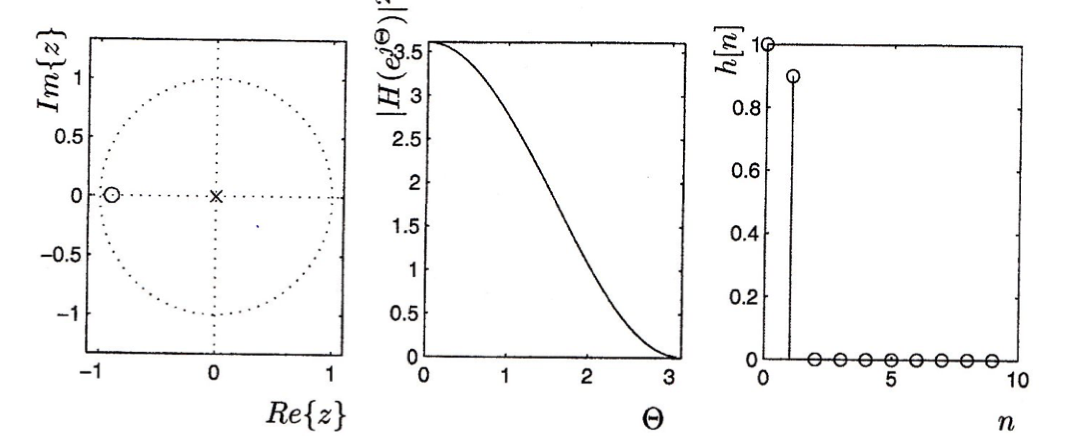
\includegraphics[width=.6\textwidth]{fig/MA_filter.png}
        \caption*{Charakteristiky filtru generujícího MA proces 1. řádu}
        \label{fig:MA:filter}
\end{figure}

\begin{figure}[h!]
        \centering
        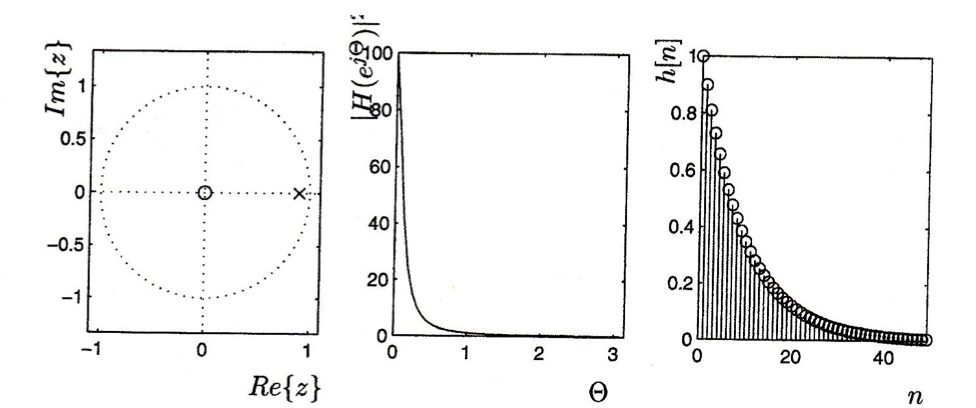
\includegraphics[width=.6\textwidth]{fig/AR_filter.png}
        \caption*{Charakteristiky filtru generujícího AR proces 1. řádu}
        \label{fig:AR:filter}
\end{figure}
\FloatBarrier

Dává smysl, že má MA ostrá minima a plochá maxima. Jelikož v MA procesu hýbeme pouze nulami, které stahují charakteristiku filtru dolu. Naopak u AR filtru hýbeme umístěním pólů, které nám zvedají charakteristiku a proto máme ostrá maxima. ARMA proces je jejich kombinací a tedy můžeme charakteristiku ovlivňovat jak nulami, tak póly. 


%6
\subsection{Proč je výhodné AR spektrální hustotu používat? Jak se liší AR spektrální hustota od spektrální hustoty určeného pomocí Fourierovy transformace? Pokuste se načrtnout typické tvary pro oba přístupy.}
Frekvenční rozlišení AR spektra (LP spektra) téměř nezávisí na délce signálu, tedy lze použít i pro krátké signály. 

Na následujících obrázcích jsou analýzy spektra tří sinusovek vytvořená pomocí DFT a AR spektra\\
{Čisté sinusovky:\\
\begin{figure}[!htb]
        \centering
        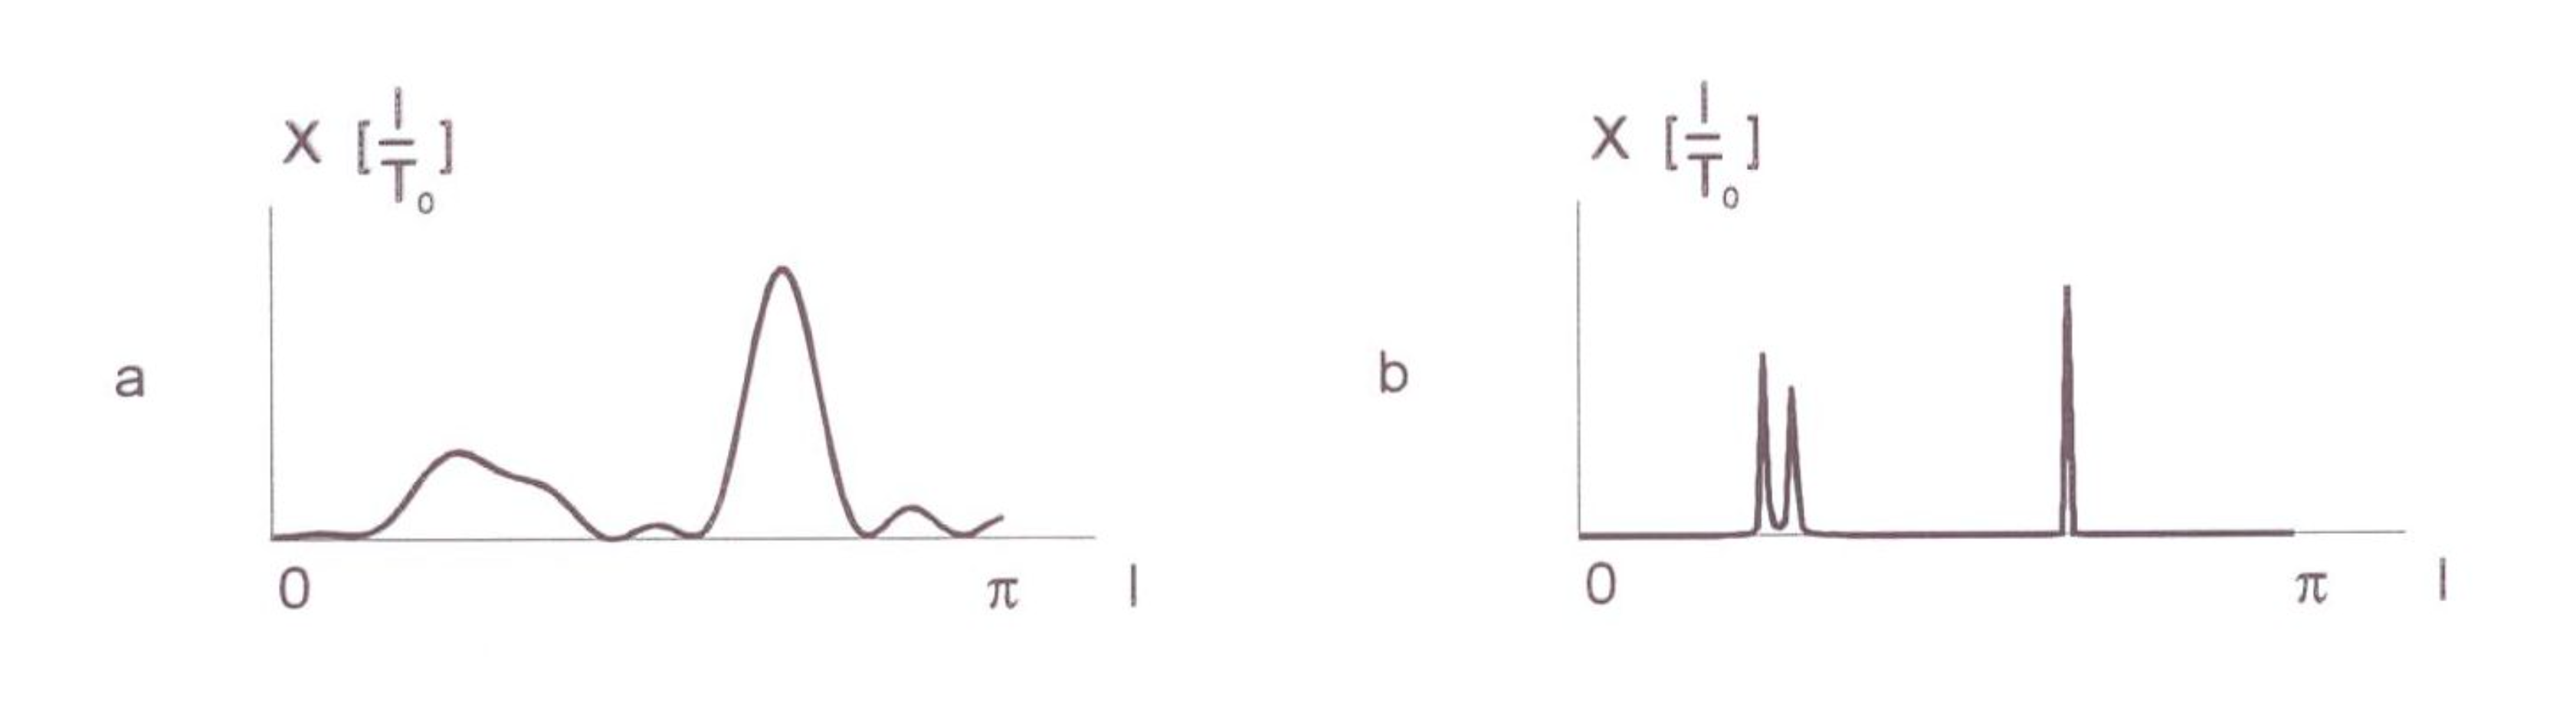
\includegraphics[width=.6\textwidth]{fig/DFT_clean.png}
        \caption*{Spektrum pomocí DFT\\ vlevo krátký segment, vpravo dlouhý}
\end{figure}
\begin{figure}[!htb]
        \centering
        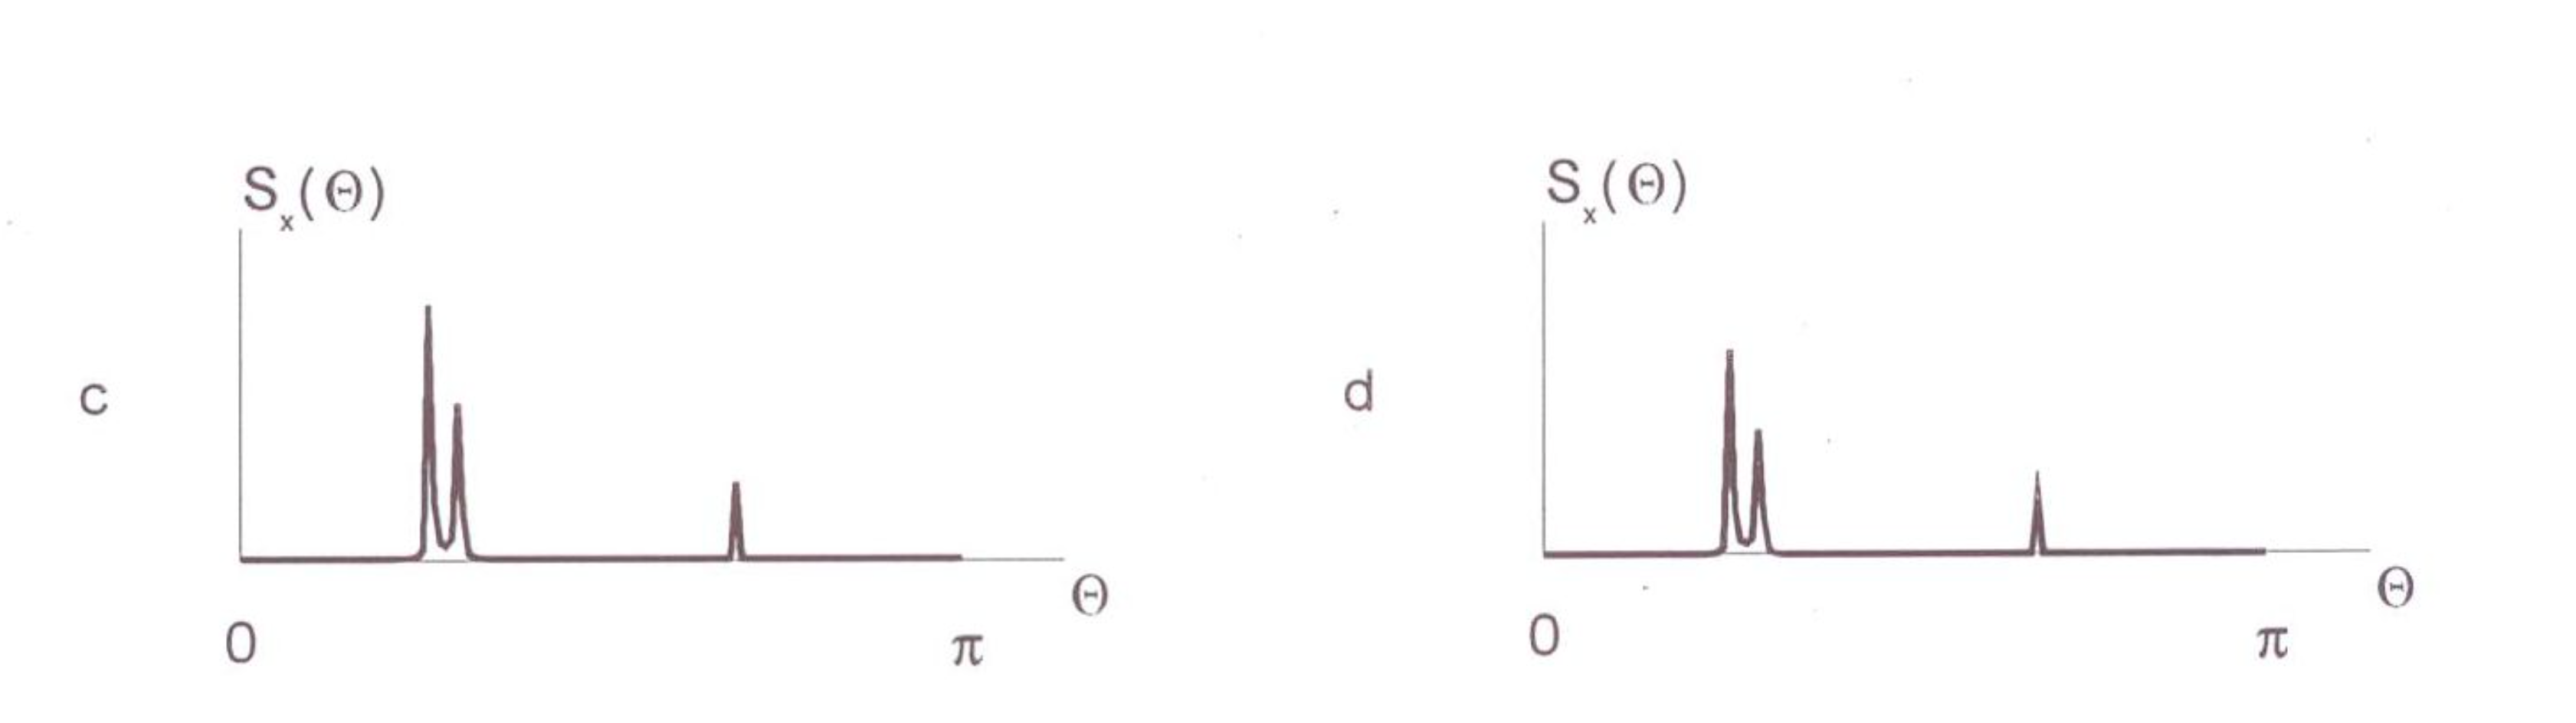
\includegraphics[width=.6\textwidth]{fig/AR_clean.png}
        \caption*{Spektrum pomocí AR\\ vlevo krátký segment, vpravo dlouhý}
\end{figure}}
\FloatBarrier
Sinusovky v šumu (SNR=0 dB)\\
\begin{figure}[h!]
        \centering
        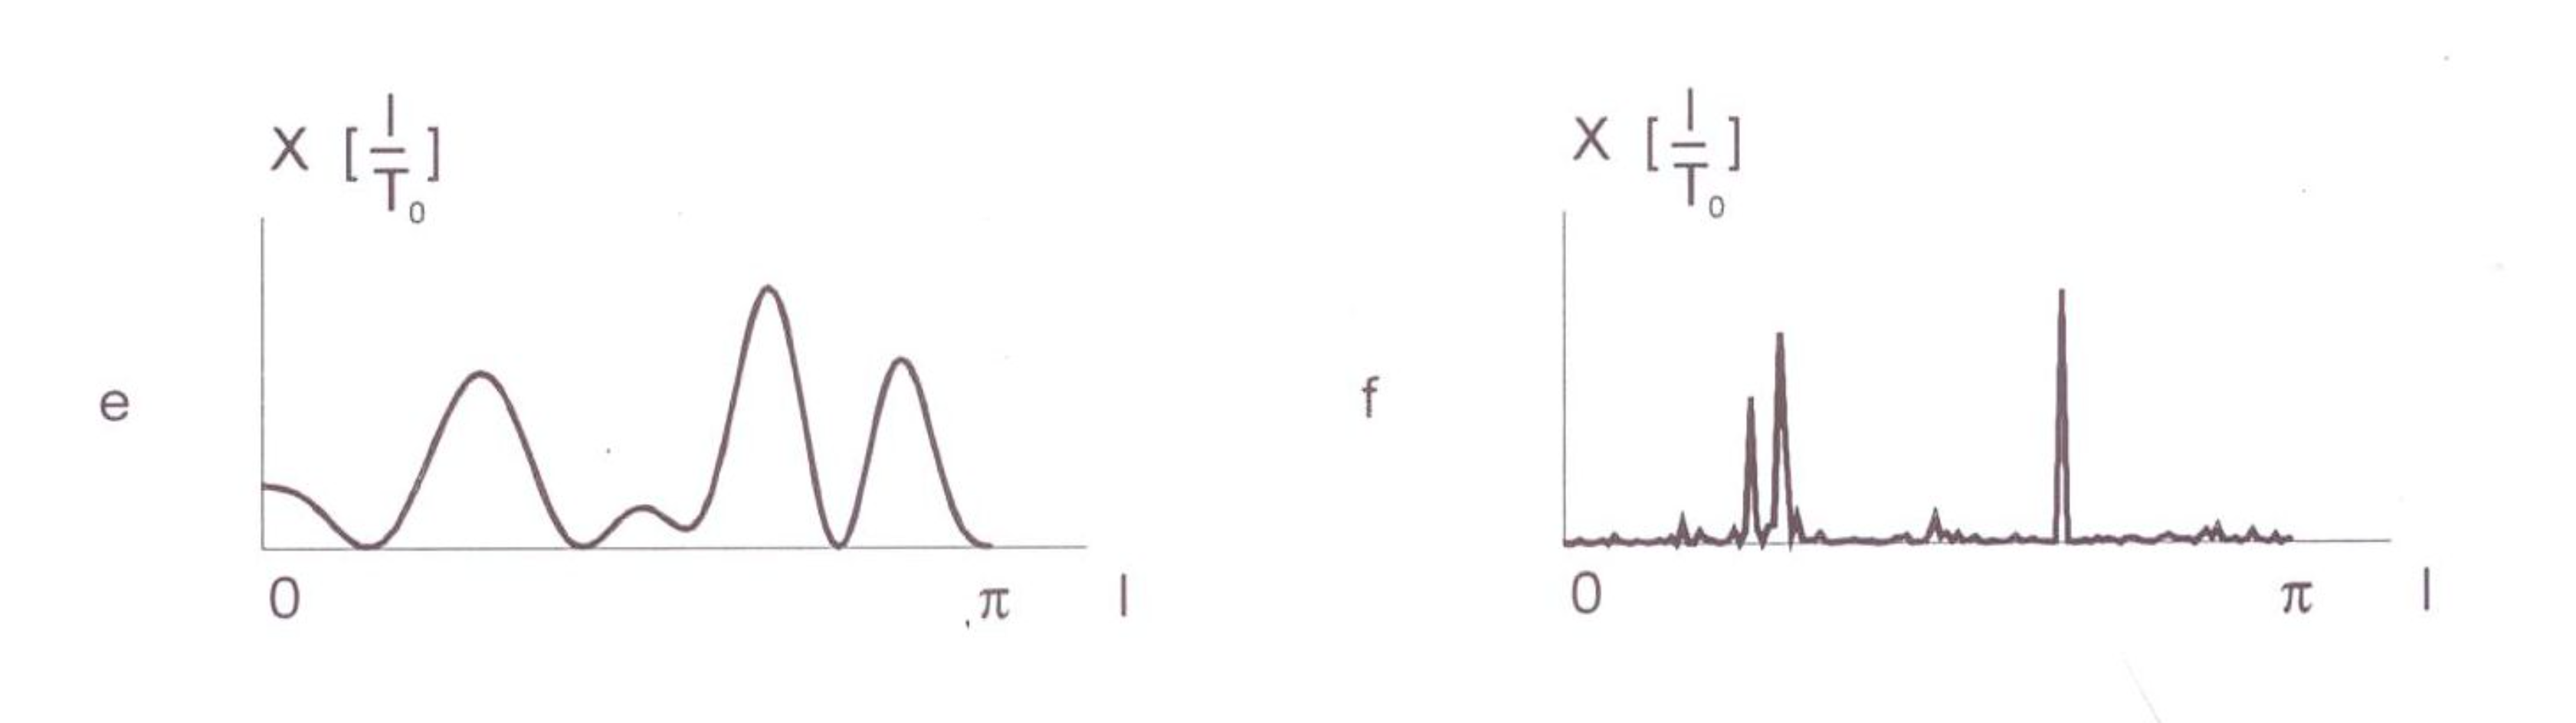
\includegraphics[width=.6\textwidth]{fig/DFT_noise.png}
        \caption*{Spektrum pomocí DFT\\ vlevo krátký segment, vpravo dlouhý}
\end{figure}
\begin{figure}[h!]
        \centering
        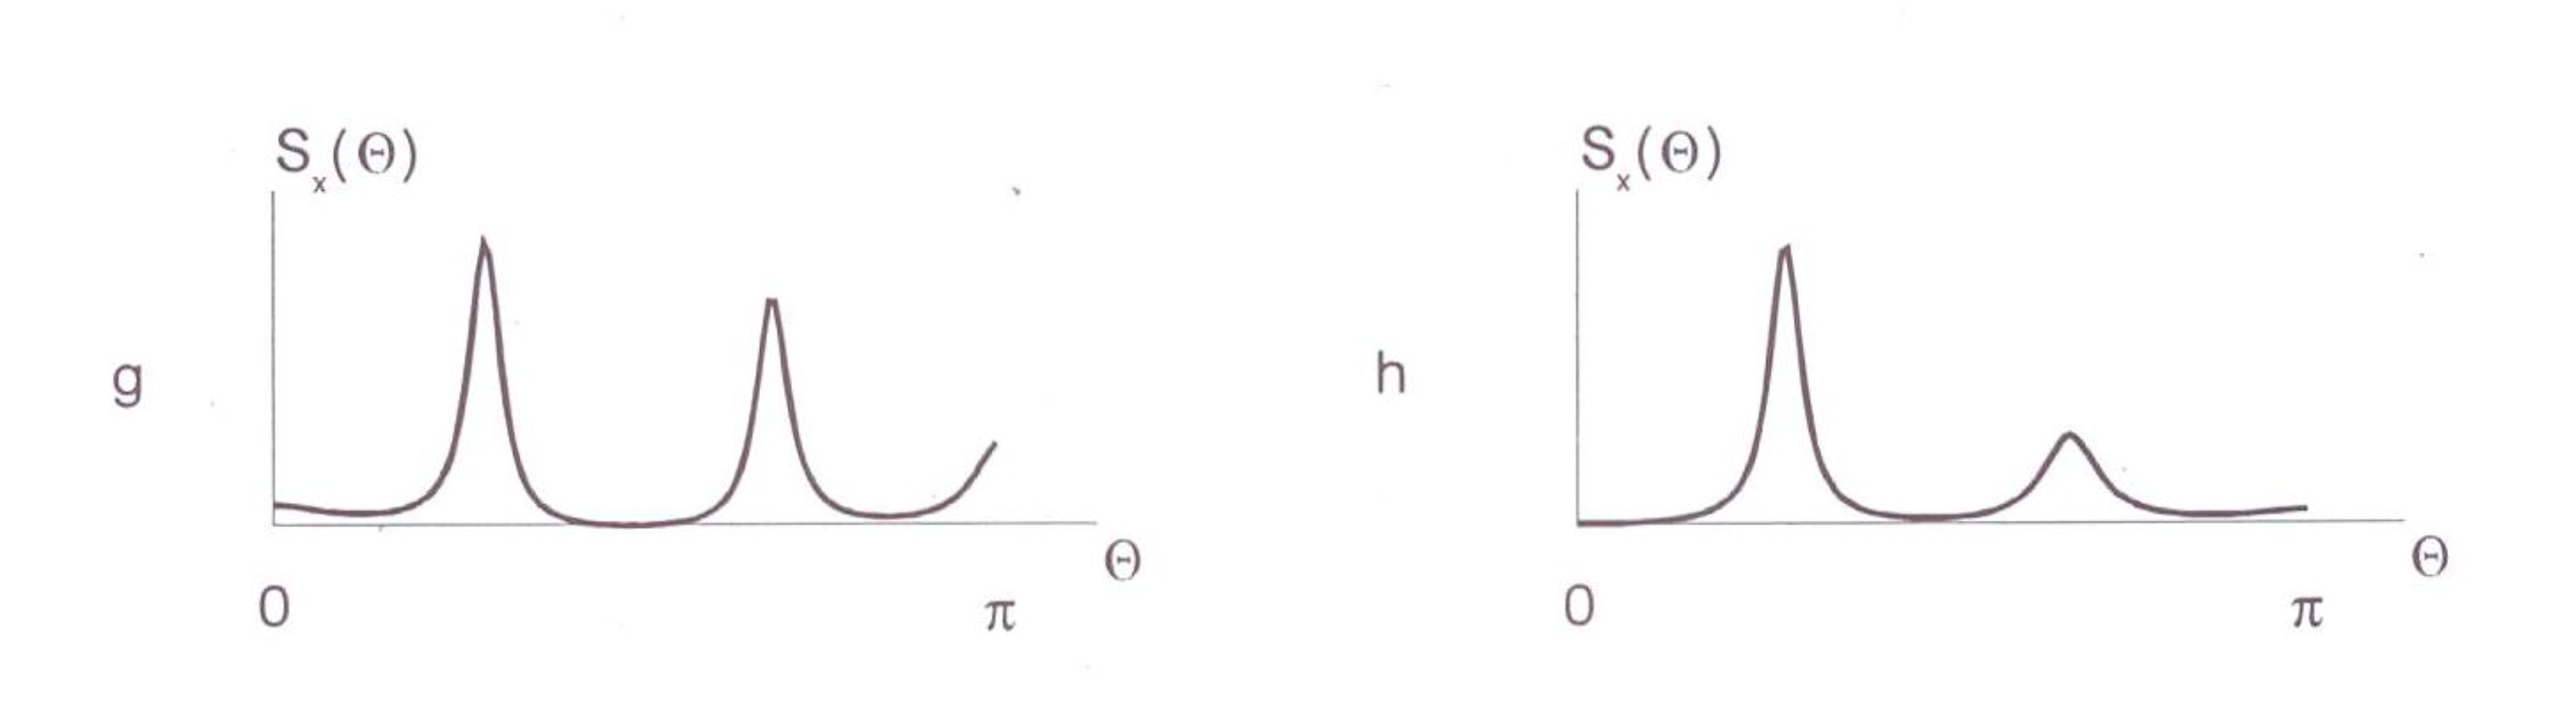
\includegraphics[width=.6\textwidth]{fig/AR_noise.png}
        \caption*{Spektrum pomocí AR\\ vlevo krátký segment, vpravo dlouhý}
\end{figure}
\FloatBarrier


%7
\subsection{Jak souvisí AR model s číslicovými filtry a číslicovou filtrací? Nakreslete příklad generování AR signálu s využitím příslušného číslicového filtru a načrtněte odpovídající tvar AR spektrální hustoty.}
AR  bude mít ostré kope a mělká údolí.

AR(p) proces lze generovat IIR filtrem řádu \mt{p}, který nemá dopředné vazby (\mt{u[n]} je bílý šum):
\begin{align*}
        x[n] = -\sum^p_{k=1}a_k x[n-k] + u[n]
\end{align*}
Bacha na mínus před sumou.

Přenosová funkce tohoto filtru je:
\begin{align*}
        H(z) = \frac{1}{A(z)} = \frac{1}{1+\sum_{k=1}^p a_k z^{-k}} = \frac{z^p}{z^p + \sum_{k=1}^p a_k z^{p-k}}
\end{align*}
Tenhle vzoreček byl už v otázce \ref{sec:ar:intro} \uv{\textit{Vysvětlete, co znamená pojem autoregresní (AR) proces}}.


%á
\subsection{Předpokládejte, že máte signál, který odpovídá AR modelu. Jak zjistíte parametry tohoto modelu? Načtrtněte blokové schéma analýzy a popište jej.}
Parametry lze zjistit pomocí Yuleovy-Walkerovy metody viz. \ref{sec:yule}. 

\textbf{Analýza signálu} \mt{x[n]}

Chybový signál \mt{e[n]}:
\begin{align*}
        e[n] = x[n] + \sum_{k=1}^M a_k x[n-k],~n=0,\,1,\,2...
\end{align*}

\begin{figure}[h!]
        \centering
        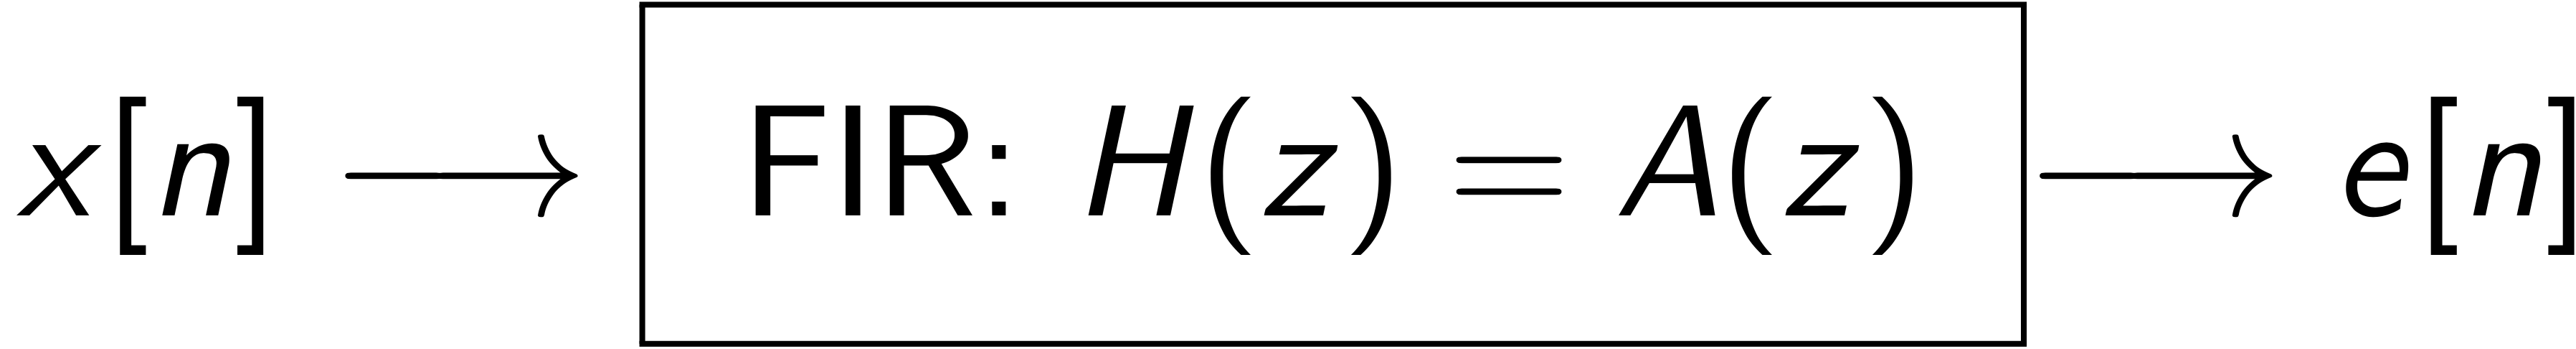
\includegraphics[width=.6\textwidth]{fig/AR_analysis_scheme.png}
        \caption*{Blokové schéma analýzy}
\end{figure}

Pokud:
\begin{itemize}
        \item \mt{x[n]} je AR signál
        \item koeficienty AR filtru jsou správně určeny
\end{itemize}
pak je chybový signál \mt{e[n]} \textbf{bílým šumem}.

\FloatBarrier

%í
\subsection{Co znamená termín lineární predikce? Co je chyba predikce? Co znamená termín dekorelace signálu a dekorelační (bělicí) filtr? Jak získáme jeho koeficienty?}\label{sec:lin:predikce}

Na základě minulých dat dokážeme sestavit AR model pro predikci budoucích dat. Analyzovaná data musí být stacionární (nemění se statistické vlastnosti s časem).

\textbf{Predikce}
\begin{align*}
        \hat{x}[n] = -\sum ^M _{k=1} a_k x[n-k],
\end{align*}
kde \mt{M} je řád prediktoru a \mt{a_k} jeho koeficienty. Bacha na mínus před sumou.

\textbf{Chyba predikce}
\begin{align*}
        e[n] &= x[n] - \hat{x}[n]\\
        e[n] &= x[n] + \sum_{k=1}^M a_k x[n-k],~n=0,\,1,\,2...
\end{align*}

Pro minimalizaci chyby následně využíváme dvou metod. Buď minimalizujeme součet čtverců chyb a nebo minimalizujeme střední kvadratickou chybu:
\begin{align*}
        \text{min}&(\sum e^2[n] )\\
        \text{min}&(E[e^2[n]])
\end{align*}


%10
\subsection{Co jsou a k čemu slouží normální (Yuleovy-Walkerovy) rovnice?}\label{sec:yule}
Normální rovnice pro \textbf{autokorelační metodu}. Jedná se o sadu rovnic určenou k odhadu parametrů AR modelu. Díky čemuž můžeme učinit odhad budoucích hodnot. Pro správný odhad musí být proces stacionární stochastický a musíme znát ACF procesu. Poté YW rovnice berou ACF koeficienty a z nich tvoří koeficienty do AR modelu.
\begin{align*}
        a_1 R_x[0] + a_2 R_x[1] = -R_x[1]\\
        a_1 R_x[1] + a_2 R_x[0] = -R_x[2]
\end{align*}


%11
\subsection{Popište postup vedoucí k určení AR spektrální hustoty. V čem se liší od spektrální hustoty získané Welchovou metodou z hlediska typického tvaru, spektrálního rozlišení, potřebné délky signálu a odolnosti vůči aditivnímu šumu?}
\begin{enumerate}
        \item Stanovení modelu autoregresního procesu podle počtu minulých hodnot (řád) např. pomocí autokorelační metody
        \item Určení koeficientů autokorelační funkce.
        \item FT pro převod autokorelace na výkonové spektrum
\end{enumerate}

Ten rozdíl bude asi zase takovejhle, idk man:a následujících obrázcích jsou analýzy spektra tří sinusovek vytvořená pomocí DFT a AR spektra\\
{Čisté sinusovky:\\
\begin{figure}[!htb]
        \centering
        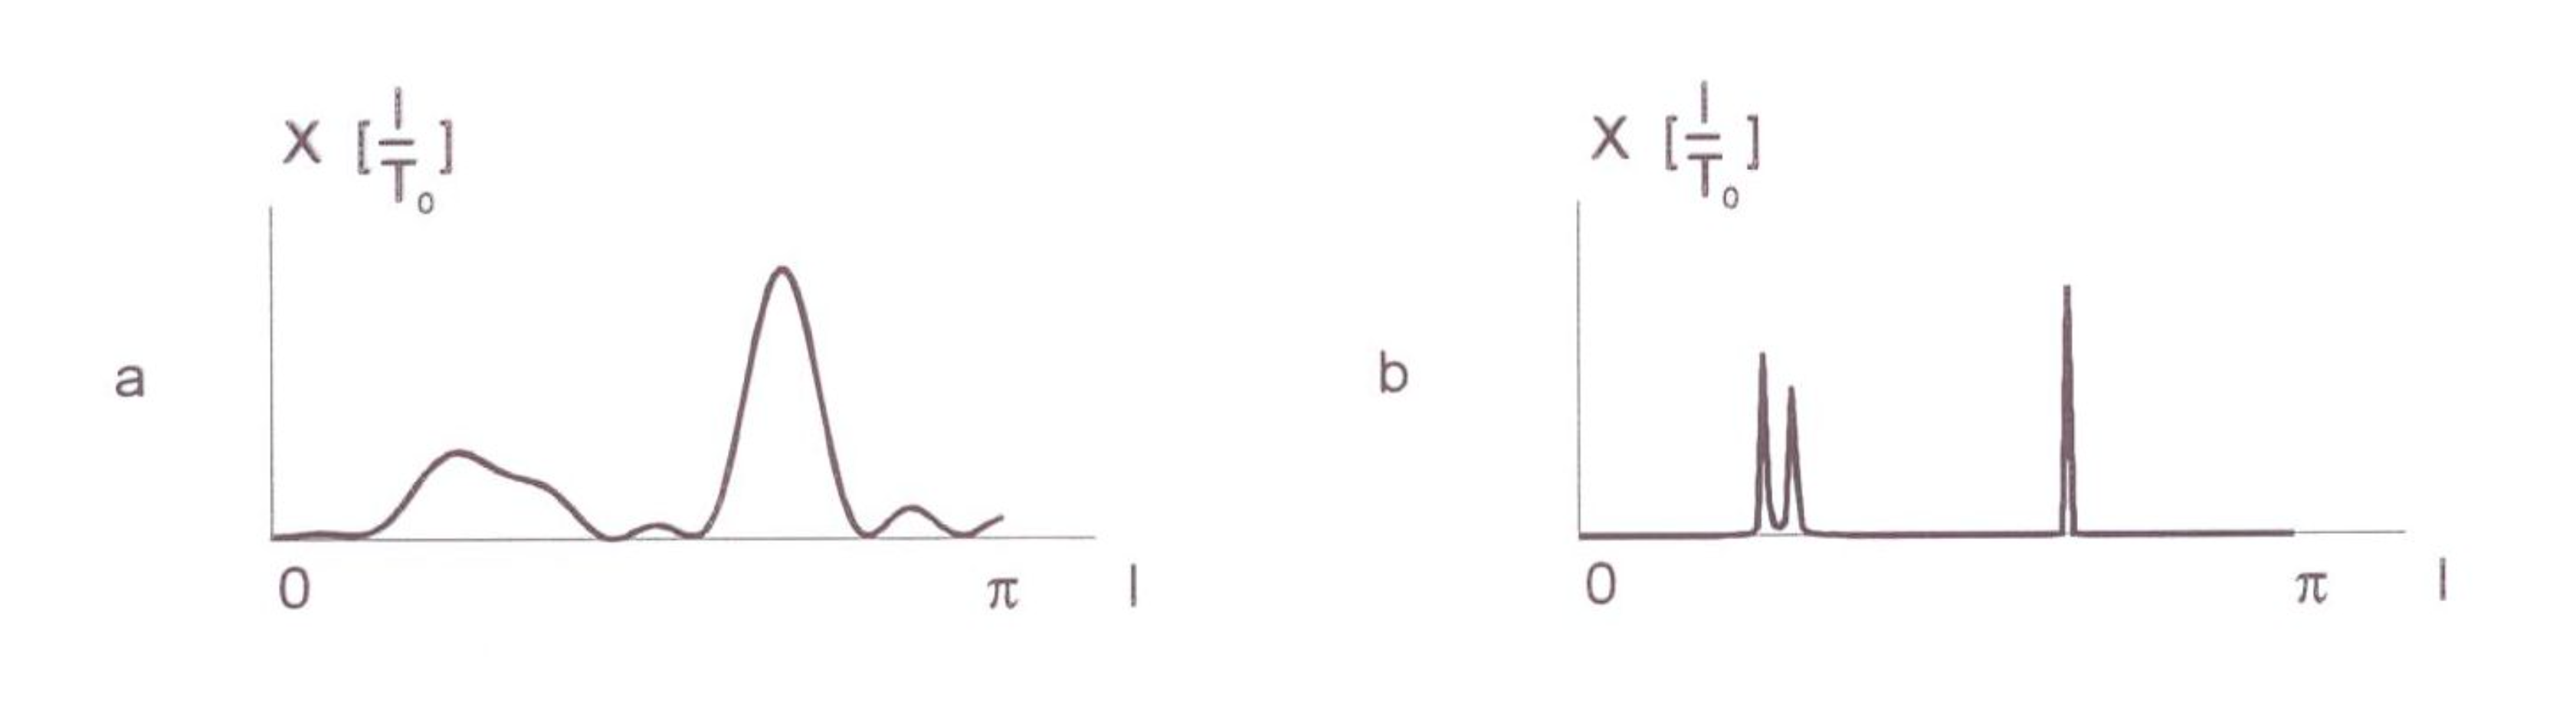
\includegraphics[width=.6\textwidth]{fig/DFT_clean.png}
        \caption*{Spektrum pomocí DFT\\ vlevo krátký segment, vpravo dlouhý}
\end{figure}
\begin{figure}[!htb]
        \centering
        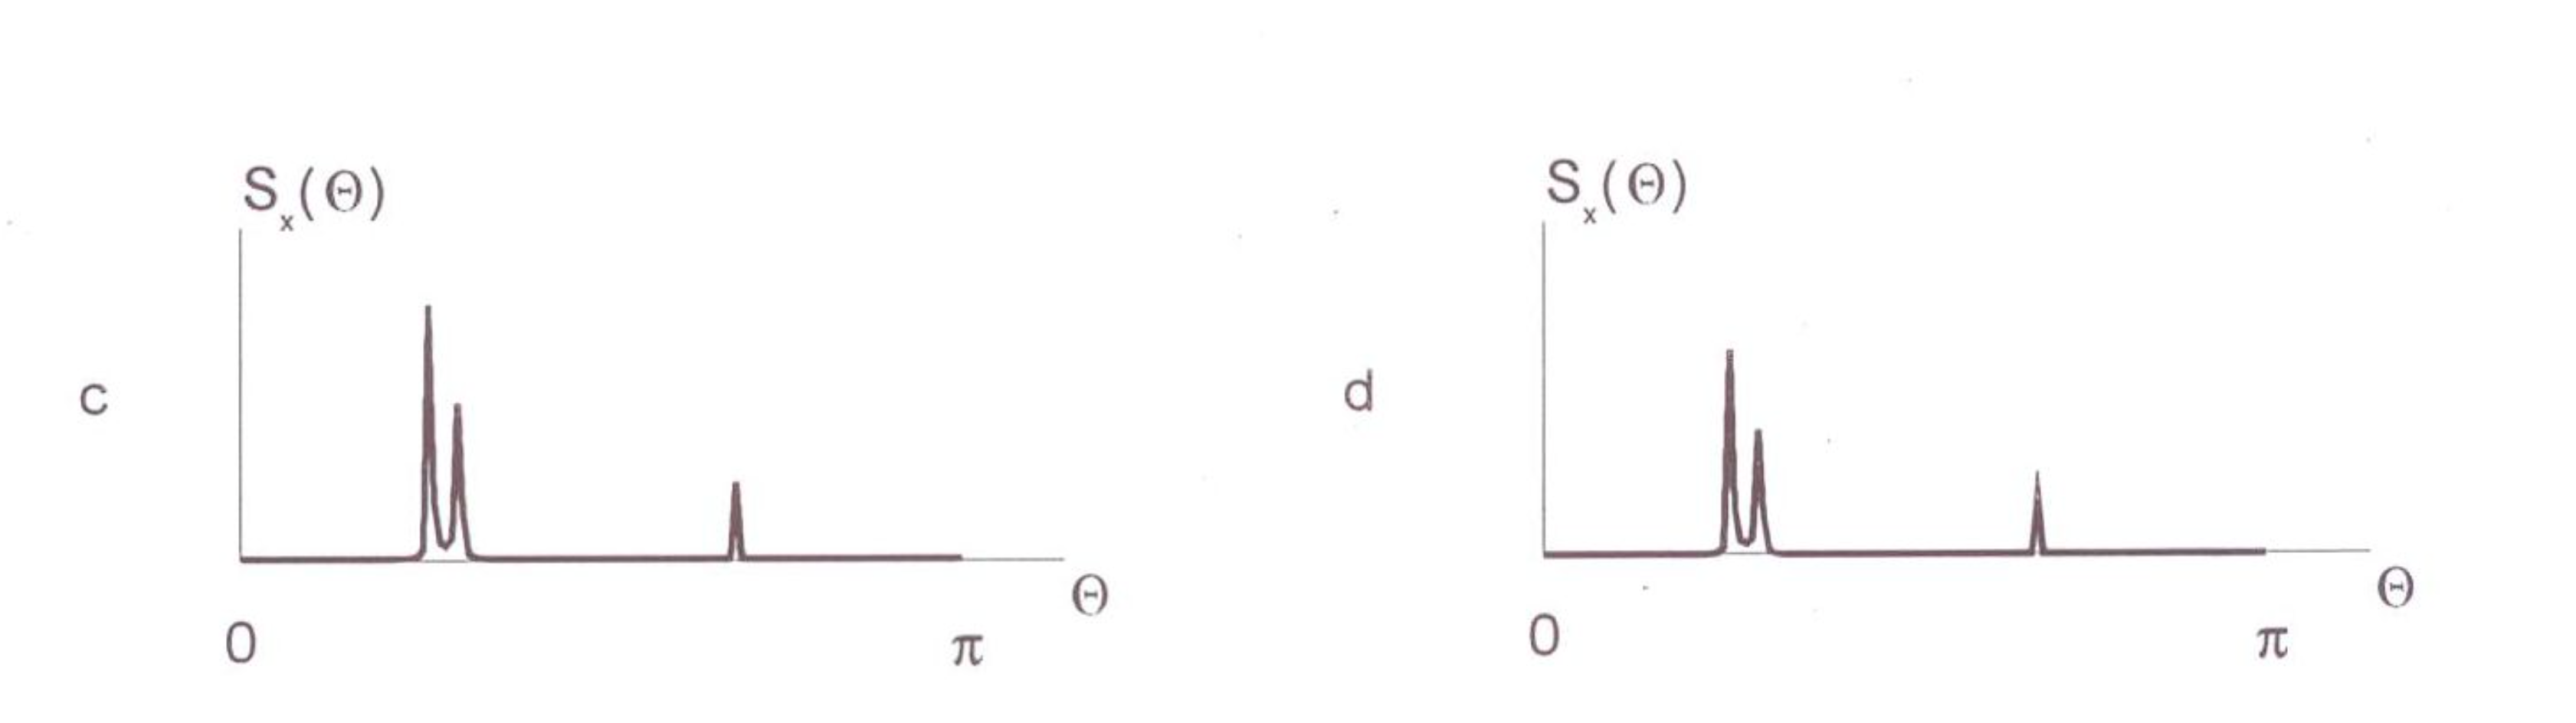
\includegraphics[width=.6\textwidth]{fig/AR_clean.png}
        \caption*{Spektrum pomocí AR\\ vlevo krátký segment, vpravo dlouhý}
\end{figure}}
\FloatBarrier
\pagebreak
{Sinusovky v šumu (SNR=0 dB)\\
\begin{figure}[h!]
        \centering
        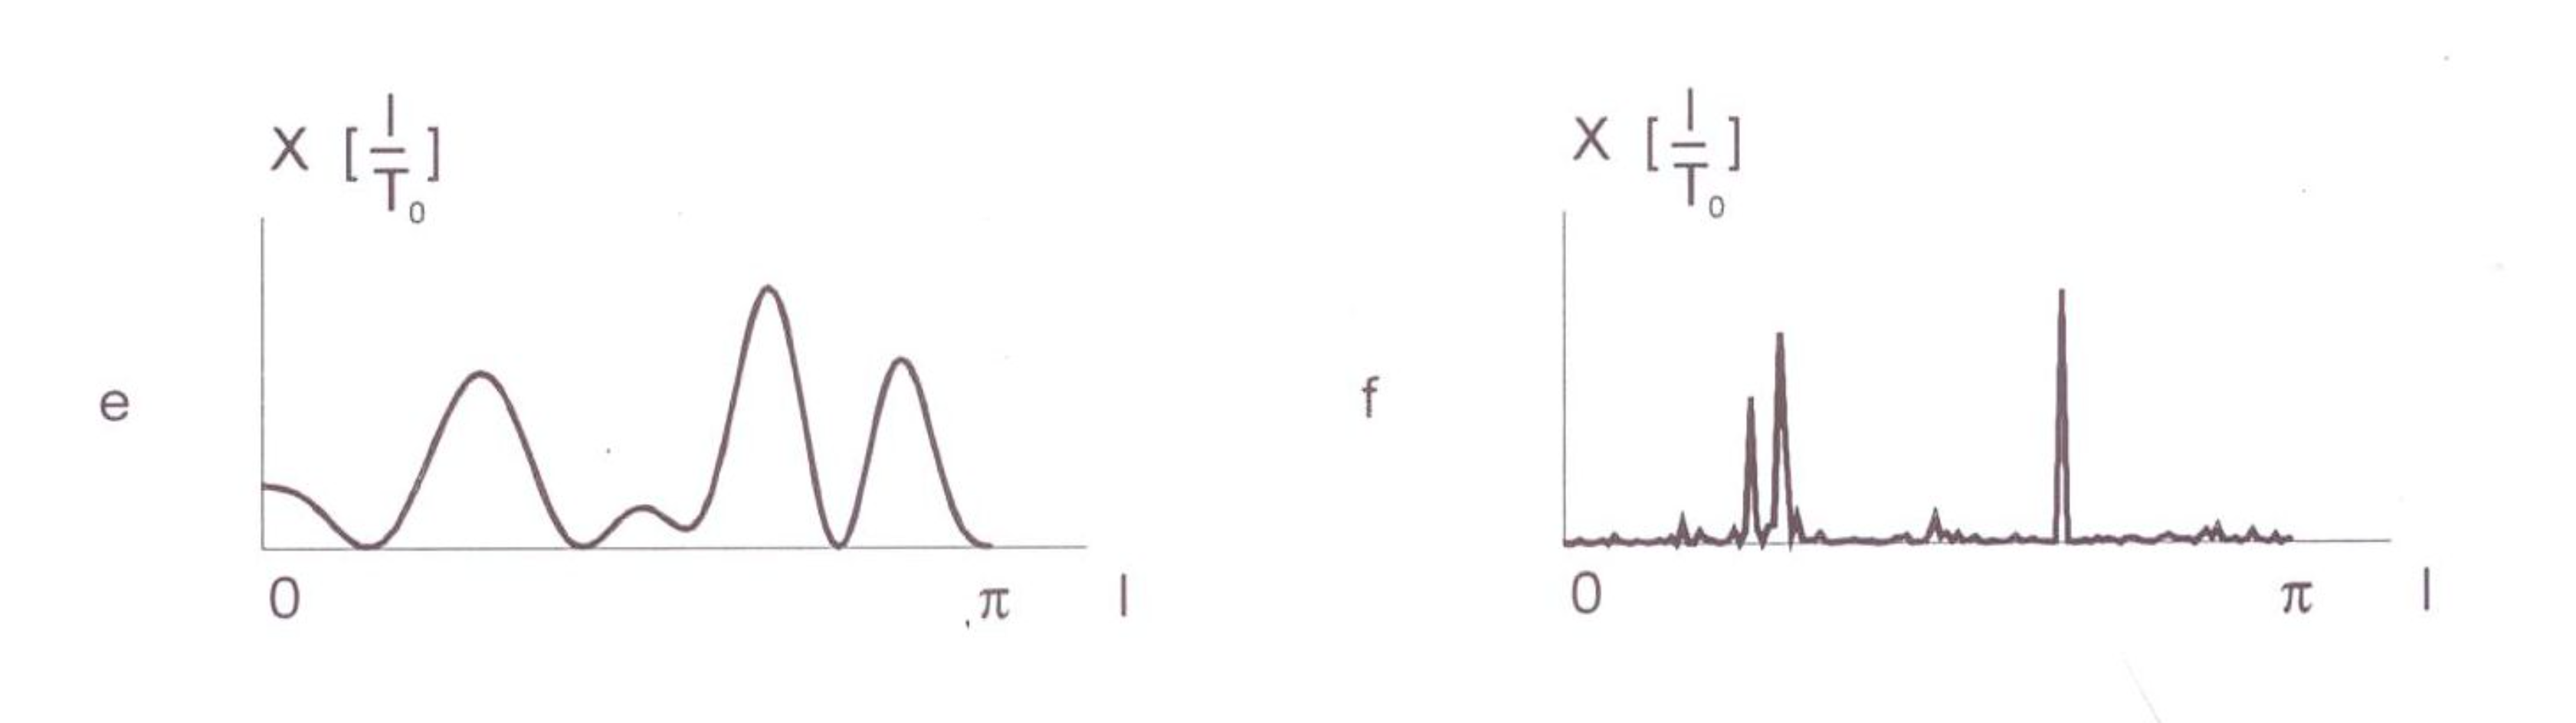
\includegraphics[width=.6\textwidth]{fig/DFT_noise.png}
        \caption*{Spektrum pomocí DFT\\ vlevo krátký segment, vpravo dlouhý}
\end{figure}
\begin{figure}[h!]
        \centering
        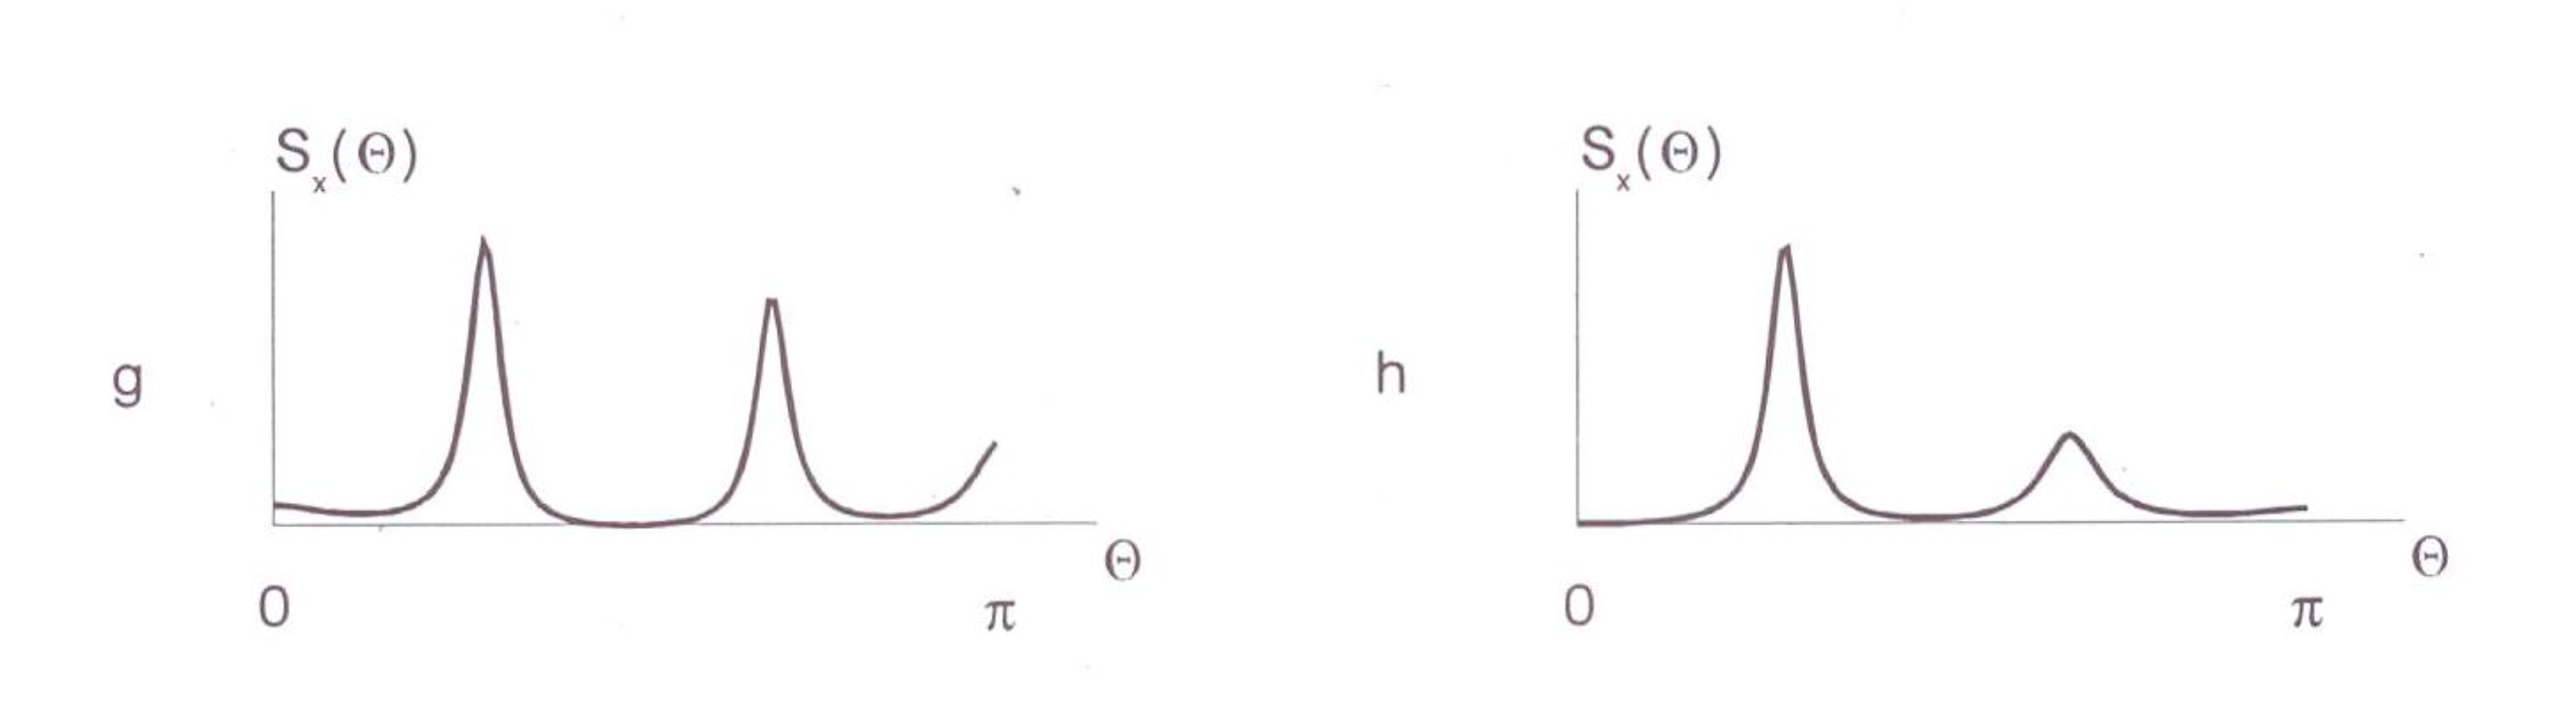
\includegraphics[width=.6\textwidth]{fig/AR_noise.png}
        \caption*{Spektrum pomocí AR\\ vlevo krátký segment, vpravo dlouhý}
\end{figure}}
\FloatBarrier





\clearpage


\section{Měření zpoždění mezi signály [12-16]} 
%12
\subsection{Co znamená termín nedisperzní a disperzní prostředí. Jak lze tato prostředí modelovat ve spojité i diskrétní oblasti? Vysvětlete a popište tato prostředí jak v časové tak i ve spektrální oblasti. Proč nás určení zpoždění mezi signály zajímá?}\label{sec:zpozdeni:uvod}


\textbf{Nedisperzní} prostředí:
\begin{outline}
        \1 frekvenčně nezávislé
        \1 zpoždění měříme korelační funkcí
        \1 konstantní útlum (\mt{k_0} signálu na všech frekvencích)
        \1 lineární fázová charakteristikami (přímka se směrnicí \mt{-\tau_0})
        \2 tedy konstantním skupinovým zpožděním (konstanta \mt{\tau_0} [s])
\end{outline}

Popis šíření ve spojitém čase:\\
\begin{align*}
        y(t) &= k_0 x (t-\tau_0)\\
        h(t) &= k_0\delta(t-\tau_0)\\
        H(p) &= k_0\e^{-\tau_0 p}\\
        H(j\omega) &= k_0\e^{-j\tau_0\omega}
\end{align*}

Popis šíření v diskrétním čase:
\begin{align*}
        y[n] &= k_0 x[n-D]\\
        H(z) &= k_0z^{-D}\\
        H(\Theta) &= k_0\e^{-jD\Theta}
\end{align*} 


\textbf{Disperzní} prostředí:
\begin{outline}
        \1 frekvenčně závislé
        \1 zpoždění měříme vzájemnou spektrální hustotou a koherencí
\end{outline}

Popis šíření:
\begin{align*}
        y(t) = x(t)\ast h(t)\rightarrow R_{xy}(\tau) = h(\tau)\ast R_{xx}(\tau)
\end{align*}
Dochází ke změně tvaru korelace mezi vstupem a výstupem, nelze použít pro měření zpoždění. 


%13
\subsection{Jaké charakteristiky lze využít pro měření zpoždění mezi signály? Jak jejich volbu ovlivňuje typ prostředí? Jaké podmínky musí být splněny pro získání spolehlivého odhadu zpoždění?}\label{sec:zpozdeni:zpusoby}

\textbf{Nedisperzní prostředí}:\\
Pokud známe vstup \mt{x(t)} i výstup \mt{y(t)}, můžeme v nedisperzním prostředí použít \textbf{vzájemnou korelaci}. Pouze v nedisperzním! V disperzním se mění tvar korelační funkce výstupního signálu a nelze tak použít. 

Jak bylo v \ref{sec:zpozdeni:uvod} uvedeno, výstupní zpožděný signál má tvar \mt{y(t) = k_0 x (t-\tau_0) + u(t)}, kde \mt{u(t)} je aditivní bílý šum.
\begin{align*}
        R_{yx}(\tau) = E[y(t+\tau)x(t)] \rightarrow k_0R_{xx}(\tau-tau_0)
\end{align*}
Nekorelovaný aditivní bílý šum nemá vliv na \mt{R_{yx}(\tau)}.

V extrému funkce \mt{R_{yx}(\tau)} najdeme zpoždění.

Pokud máme dvě cesty šíření, dostaneme dva extrémy. Rozlišitelné, pokud jsou signály širokopásmové \mt{\leftrightarrow} mají úzkou korelační funkci.

Pokud známe signály procházející dvěma a více cestami, lze získat směrový příjem.

\textbf{Disperzní prostředí}:\\
Je nutné použít vzájemnou spektrální hustotu (CPSD - Cross Power Spectral Density).
\begin{align*}
        S_{yx}(f) = \mathscr{DFT}\{R_{yx}(\tau)\} = \dots = |S_{yx}(f)|\e^{j\phi(f)}
\end{align*}
V \mt{|S_{yx}(f)|} se projeví změna tvaru korelační funkce.\\
V \mt{{j\phi(f)}} se projeví informace o zpoždění. 

Derivací fázové charakteristiky (aka skupinové zpoždění) dostaneme posun mezi signály:
\begin{align*}
        g_0(\omega) = -\frac{\dd \phi_{xy}(\omega)}{\dd \omega}
\end{align*}

Tato metoda lze použít jak pro disperzní, tak pro nedisperzní prostředí.

Podmínky:
\begin{outline}
        \1 nutno použít vyhlazenou PSD, nikoliv periodogram
        \1 pokud je fáze PSD nelineární, zpoždění je frčně závislé
        \1 při vícecestném šíření jsou spektra násobena hřebenovou frční charakteristikou (problémos)
\end{outline}



%14
\subsection{Jak vypadá vzájemná korelace mezi signálem na vstupu a na výstupu LTI soustavy? Jaký je její vztah k autokorelaci vstupního signálu?}
Vzoreček zmíněn ve \ref{sec:zpozdeni:zpusoby}.
\begin{align*}
        R_{yx}(\tau) = E[y(t+\tau)x(t)] \rightarrow k_0R_{xx}(\tau-\tau_0)
\end{align*}

Rozdíl mezi \mt{R_{yx}} a \mt{R_{xx}} je pouze ve zpoždění \mt{\tau_0}.


%15
\subsection{Jak lze ze vzájemné korelační funkce určit zpoždění mezi vstupním a výstupním signálem LTI soustavy? Načrtněte obrázek a pomocí něj vysvětlete. Jak souvisí toto zpoždění se vzorkovací frekvencí?}
Popsáno v \ref{sec:zpozdeni:uvod} a \ref{sec:zpozdeni:zpusoby}. Najdeme si maximum korelace mezi vstupem a výstupem. Z pozice maxima vzájemné korelace získáme, o kolik vzorků jsou od sebe signály posunuté.


%16
\subsection{Jaký vliv má aditivní šum, který působí na výstupu soustavy a je nekorelovaný se signálem na výpočet vzájemné korelace a tedy odhad zpoždění?}
Řečeno v \ref{sec:zpozdeni:uvod}, aditivní bílý šum \textbf{nemá vliv} na výpočet zpoždění. 

Jelikož je podmínka \uv{nekorelovaný šum}, musí platit
\begin{align*}
        E[x(t)u(t)] = 0
\end{align*}
Pro vzájemnou korelaci vstupu a výstupu můžeme psát
\begin{align*}(
        R_{yx}(\tau) = E[y(t+\tau)x(t)] + E[u(t+\tau)x(t)] = k_0R_{xx}(t-\tau_0) + 0 
\end{align*}


%17
\subsection{V jakém vztahu jsou autospektrální spektrální hustoty signálu na vstupu a na výstupu LTI soustavy? Jak lze vyjádřit vzájemnou spektrální hustotu (CPSD) mezi vstupem a výstupem LTI systému?} \label{sec:zpozdeni:SyxRyx}

Zmíněno v \ref{sec:zpozdeni:zpusoby}:
\begin{align*}
        S_{yx}(f) = \mathscr{DFT}\{R_{yx}(\tau)\} = \dots = |S_{yx}(f)|\e^{j\phi(f)}
\end{align*}

Vztah mezi vstupem a výstupem:
\begin{align*}
        S_{yx}(f) = H(f) S_{xx}(f) 
\end{align*}



%18
\subsection{Porovnejte výhody a nevýhody měření zpoždění mezi signály pomocí vzájemné korelační funkce a fáze vzájemné spektrální hustoty – jaké jsou podmínky správného měření? Proč se pro měření zpoždění používá fáze a nikoliv modul CPSD?}
Úvod v \ref{sec:zpozdeni:zpusoby}.\\
\textbf{Vzájemná korelační funkce}:
\begin{outline}
        \1 pouze pro nedisperzní prostředí 
        \1 signál musí být širokopásmový a neperiodický
        \1 rozlišení závisí na \mt{f_s}
        \1 jednoduché
\end{outline}

\textbf{CPSD}:
\begin{outline}
        \1 lze pro disperzní i nedisperzní prostředí
        \1 náchylné na šum (je potřeba používat vyhlazenou spektrální hustotu)
        \1 pokud je fáze PSD frčně závislá, tak je i zpoždění frčně závislé
\end{outline}

U CPSD je informace o zpoždění zakódovaná ve fázi (viz \ref{sec:zpozdeni:SyxRyx}).





%%%%%%%%%%%%%%%%%%%%%%%%%%%%%%%%%%%%%%%%%%%%%%%%%%%%%%%%%%%%%%%%%%%%%%%%%%%%%%%%%
\newpage \section{Koherenční funkce}
%19
\subsection{Definujte koherenční funkci a vysvětlete její význam. Jak se liší od korelačního koeficientu?}
Koherenční funkce - normovaná CPSD
\begin{equation}
        \gamma_{yx}(f) = \frac{S_{yx}(f)}{\sqrt{S_{xx}(f)S_{yy}(f)}}
\end{equation}
Komplexní funkce, lze využít pro měření zpoždění.

Koherenční funkce \mt{\gamma_{yx}} odpovídá korelačnímu koeficientu \mt{r_{yx}} s tím rozdílem, že:
\begin{outline}
        \1 \mt{\gamma_{yx} \in \mathbb{C}, r_{yx} \in \mathbb{R}}
        \1 korelační koeficient není funkcí frekvence
\end{outline}

Korelační koeficient:
\begin{align*}
        r_{yx} = \frac{\sigma_{yx}}{\sqrt{\sigma_x^2}\sqrt{\sigma_y^2}}
\end{align*}


%20
\subsection{Jak se MSC (kvadrát modulu koherenční funkce) liší od koherenční funkce?}

MSC je  kvadrát modulu koherenční funkce (koherenční funkce je normovaná CPSD)

Definice:
\begin{align*}
        C_{yx}(f) = MSC_{yx}(f) = |\gamma_{yx}(f)|^2 = \frac{|S\yx (f)|^2 }{S\xx (f)S\yy (f)} ~\in \mathbb{R}.
\end{align*}

Vlastnosti MSC
\begin{outline}
        \1 nabývá hodnot <0,1>
        \1 vypovídá o podobnosti (korelaci) signálů v jednotlivých frekvenčních pásmech
        \1 normovaná vzájemná spektrální hustota
        \1 komplexní fce reálné frekvence
        \1 od korelačního koef. se liší tak, že korelační koef. se počítá pro dva signály a pro celé spektrum, ale koherenční fce je pro jednu danou frci
        \1 koherenční fce v amplitudě 0 .. 1, korelační koef. - 1 .. 1
\end{outline}


CPSD \rrarr \textit{normování} \rrarr koherenční funkce \rrarr \textit{modul kvadrát} \rrarr MSC


%21
\subsection{K čemu se MSC používá a jaké má vlastnosti z hlediska šumu, nelinearity systému a chyb měření?}

Umožňuje odhadnout chybu měření, frekvenční charakteristiky, jestli je přítomen šum, nelinearita systému.

Příčiny nízké hodnoty MSC
\begin{outline}
        \1 chyba odhadu - nízký počet průměrování, nízké spektrální rozlišení (krátké okno)
        \1 podobnost signálů ve frekvenčním spektru je nízká
        \1 nelineární závislost mezi \mt{x} a \mt{y}
        \1 přítomnost šumu na vstupu/výstupu
        \1 jedná se o MIMO systém
\end{outline}


%22
\subsection{Jak se správně provede odhad MSC? Vysvětlete co se stane, když je použit nesprávný postup.}

Welchova metoda, vzájemná spektrální hustota - \textbf{nejdříve průměrování} a pak až kvadrát modulu. Bez průměrování dostaneme MSC = 1 !!
\begin{figure}[h!]
        \centering
        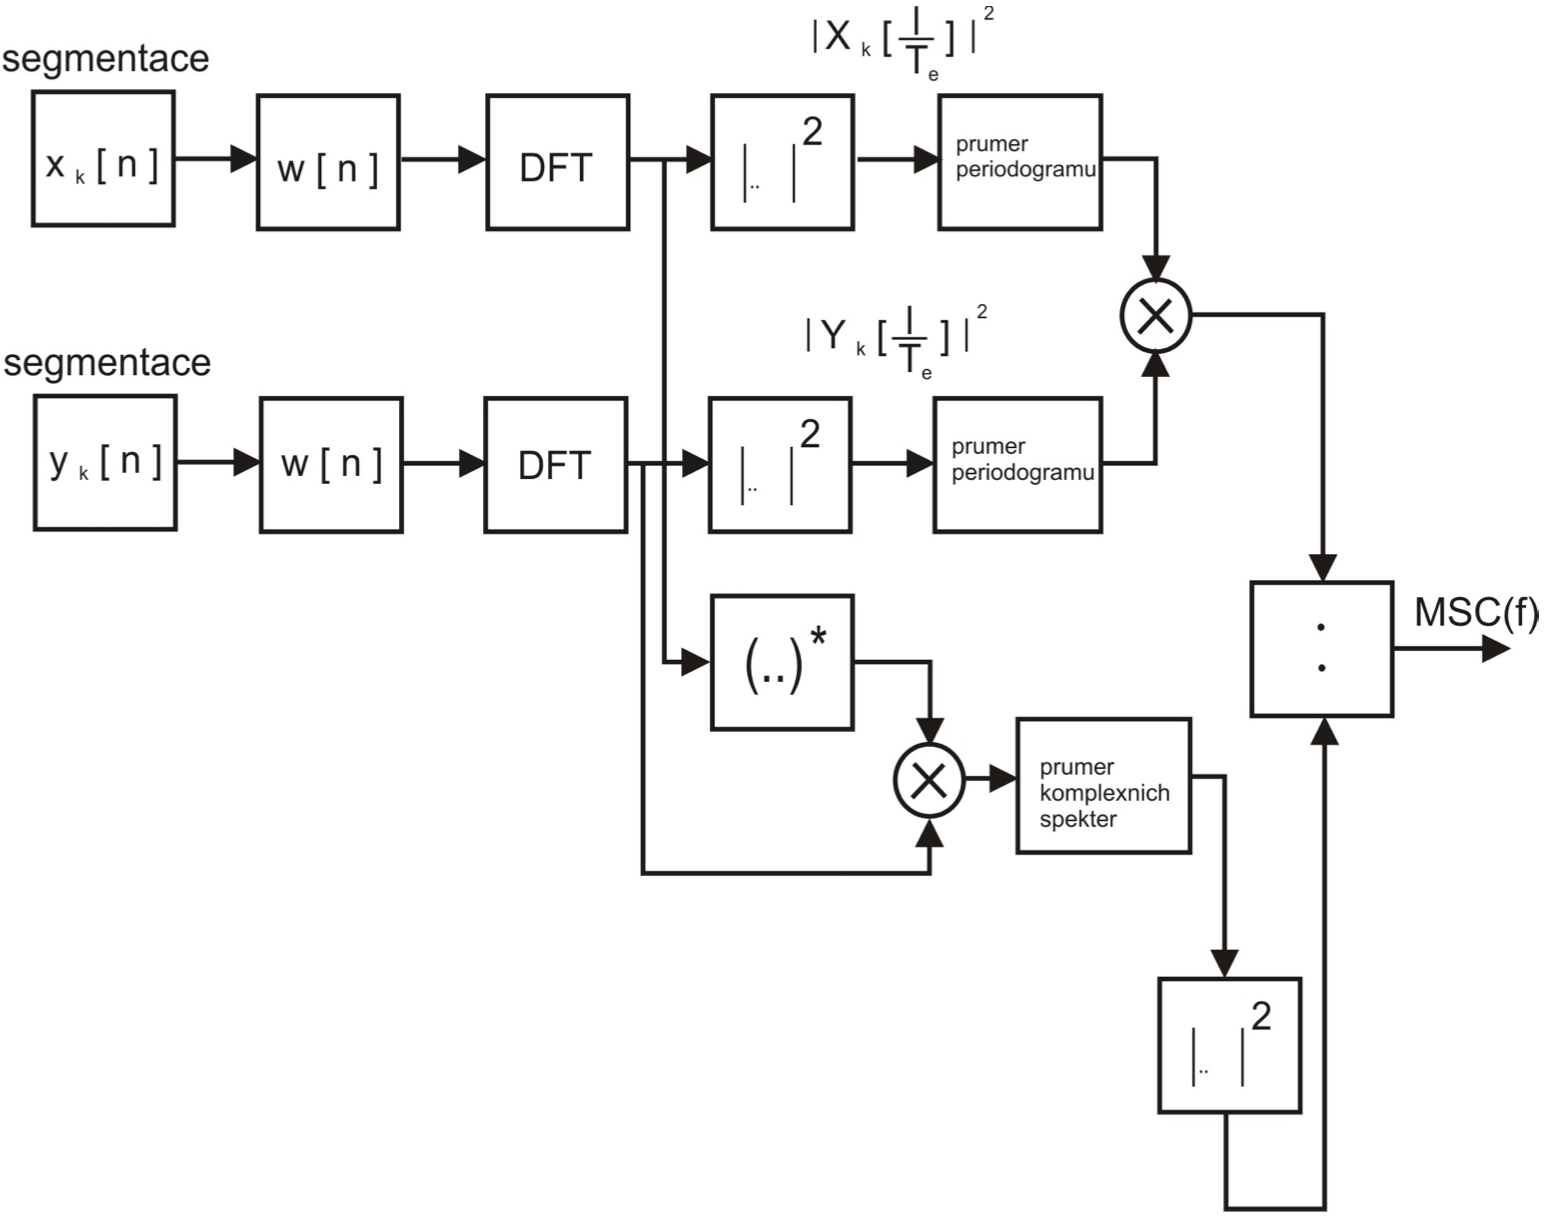
\includegraphics[width=.7\textwidth]{fig/MSC_blokove_schema.png}
        \caption*{Blokové schéma výpočtu MSC}
\end{figure}
\FloatBarrier


%23
\subsection{Jak se projeví aditivní šum na vstupu i výstupu soustavy, který je nekorelovaný se signálem, na hodnotě MSC? Jak se projeví filtrace signálu na hodnotě MSC?}

Hodnota MSC se sníží. MSC říká, jaká část spektrální čáry je generovaná vstupem a jak á je generovaná šumem. Lin f nemůže MSC snížit. Pokud aditivní šum, sníží se. Nelineární filtr - sníží se. Pokud ale dostatečně dlouhý stac. signál

I když přidáme na výstup šum \mt{m(t)}, bude platit \mt{S_vx(f) = S_yx(f)}, protože platí \mt{R_vx = R_yx} \llarr bílý šum neovlivní korelaci (řekli jsme, že je nekorelovaný). 


%24
\subsection{Lze koherenci použít pro odhad zpoždění mezi signály?}

Ano. Ne přímo skrze MSC, ale přes koherenční fci - zjistíme z fáze. Koherenční fce \uv{jen} normovaná CPSD. Jednodušší je ale rovnou použít PSD \mt{S_x}.


\newpage \section{Kepstrální analýza a její aplikace, míry}
%25
\subsection{Vysvětlete princip superpozice a zobecnělý princip superpozice. Co znamená pojem konvoluce a dekonvoluce. Jak lze provést dekonvoluci při znalosti vstupního a výstupního signálu a co je výsledkem této dekonvoluce?}
Odezvy více složek systému lze rozdělit na jednotlivé odezvy a poté sečíst. Transformace součtu je součet transformací. 

\textbf{Dekonvoluce}: převedeme na spektrum a podělíme \llarr dekonvoluce wow. 


%26
\subsection{Lze provést dekonvoluci pouze ze znalosti výstupního signálu LTI systému? Jaké podmínky je třeba splnit, aby tato úloha měla řešení?}

Ano, pomocí kepstrální analýzy.

Podmínky:
\begin{outline}
        \1 jedna ze složek musí být aperiodická (impulz)
        \1 druhá se musí chvíli periodicky opakovat
\end{outline}


%27
\subsection{K čemu se kepstrální analýza používá? Je to lineární nebo nelineární metoda analýzy?}

Dekonvoluce signálů, nelineární (logaritmus)


%28
\subsection{Vyjmenujte tři základní bloky používané pro kepstrální analýzu a rekonstrukci signálu.}

\mt{\mathscr{Z}, \mathscr{DFT}, \mathscr{DTFT} \rightarrow \text{log, exp }\rightarrow \mathscr{Z}^{-1}, i\mathscr{DFT}, i\mathscr{DTFT}}


%29
\subsection{Jakými operacemi se realizují základní bloky kepstrální analýzy při použití DFT?}

\mt{\mathscr{Z}, \mathscr{DFT}, \mathscr{DTFT} \rightarrow \text{log, exp }\rightarrow \mathscr{Z}^{-1}, i\mathscr{DFT}, i\mathscr{DTFT}}


%30
\subsection{Jakými bloky a operacemi se realizují základní bloky rekonstrukce signálu při použití DFT?}

Viz předchozí.


%31
\section{Co je liftrace a k čemu slouží?}

Oříznutí kepstra, které je součet periodické a aperiodické složky. Normálně by to byl součin, ale díky logaritmu je to součet. Blíže k nule je to aperiodická složka, dále od nuly periodická. Osa x se jmenuje \textit{kvefrence}. (:.


%32
\subsection{Jakou informaci nese kepstrum na nízkých frekvencích a jakou na vysokých?}

Nízké - aperiodické složky signálu\\
Vysoké - periodické složky


%33
\subsection{Proč kepstrum dokáže odhalit i slabý odraz?}

Protože kepstrální analýza zatlumí impuluz a zatlumení je dáno posloupností \mt{1/n}.


%34
\subsection{Jaký je vztah mezi spektrem, logaritmickým spektrem, autokorelační funkcí a kepstrem?}

ACF::\\
\mt{x[n] \rightarrow \mathscr{DFT} \rightarrow \frac{1}{N}|\dots|^2 \rightarrow i\mathscr{DFT} \rightarrow R_x[k]}
\begin{align*}
        R[n] = \frac{1}{2}\frac{1}{2\pi j}\oint (X(z)X(z^{-1}))z^{n-1}\dd z
\end{align*}


Reálné kepstrum:\\
\mt{x[n] \rightarrow \mathscr{DFT} \rightarrow \frac{1}{N}|\dots|^2 \rightarrow \ln (...) \rightarrow i\mathscr{DFT} \rightarrow c_x[n]}
\begin{align*}
        c_x[n] = \frac{1}{2}\frac{1}{2\pi j}\oint \underline{\ln}(X(z)X(z^{-1}))z^{n-1}\dd z
\end{align*}



Komplexní kepstrum
\begin{align*}
        \hat{x}[n] = \frac{1}{2\pi j}\oint \ln(X(z))z^{n-1}\dd z
\end{align*}




%35
\subsection{Lze kepstrální koeficienty získat i jiným způsobem, než pomocí DFT? Vysvětlete stručně alternativní postup jejich výpočtu.}

Jo. Použitím lineární predikce LPC. Signál \mt{x[n]} nasegmentujeme, naváhujeme oknem a pošleme do LPC. Tím získáme AR koeficienty. Liší se ve výpočtu spektrální výkonové hustoty. Welch (origo) nebo LPC. LPC bude mít méně detailů, jelikož budeme používat vyhlazené spektrum. 

AR koeficienty lze pomocí rekurzivní rovnice převést na kepstrální koeficienty. 


%36
\subsection{Porovnejte vlastnosti kepstra získaného pomocí DFT a pomocí AR modelu.}

AR model bude mít vyhlazenější kepstrum, ale bude náchylnější na šum.


%37
\subsection{Vyjmenujte některé aplikace kepstrální analýzy.}
\begin{outline}
        \1 dekonvoluce řeči
        \1 parametrizace řeči pro účely analýzy a rozpoznání
        \1 analýza vibrací, detekce poruch ložisek, ozubených kol\dots
        \1 detekce odrazů signálů (akustické vlastnosti místností, lokalizace diskontinuity na optickém kabelu)
        \1 získání spektrální obálky signálů
\end{outline}


%38
\subsection{Jaké vlastnosti má metrika (míra)? Jaké typy metrik a integrálních metrik znáte? Uveďte příklad vybrané metriky.}
\begin{outline}
        \1 nezáporná
        \1 symetrická
        \1 platí trojúhelníková nerovnost
\end{outline}

\textbf{Euklidovský prostor}\\
L1 - newyorkská metrika, můžeme chodit jen jako v ulicích Newyorku\\
L2 - klasická vektorová vzdálenost\\
L\mt{\infty} - Čebyšeova metrika

\textbf{Integrální metrika}\\
Metrika v prostoru spojitých funkcí


%39
\subsection{Definujte spektrální vzdálenost. Souvisí tato metrika s kepstrální vzdáleností?} 
Integrál absolutní hodnoty rozdílu dvou ln(PSD)
\begin{align*}
        d_2^2 = \frac{1}{\pi} \int _0^\pi |\ln(S_x(\theta)) - \ln(S_y(\theta))|^2\dd (\theta)
\end{align*}

Ano, souvisí. Jak, to nevím.


%40
\subsection{Jak se určí kepstrální vzdálenost pro konečný počet kepstrálních koeficientů?}

Kepstrální vzdálenost se určí ze spektrální vzdálenosti. Ze spektrálních koeficientů si spočteme kepstrální koeficienty. Kepstrální vzdálenost je poté Euklidovská vzdálenost v L-rozměrném prostoru kepstrálních koeficientů.


%41
\subsection{Shrňte vlastnosti a význam kepstrální vzdálenosti.}
\begin{outline}
        \1 Pomáhá nám posoudit, zdali dva segmenty, které zpracováváme, pocházejí ze stejného zdroje a jestli jsou korelované.
        \1 \mt{c_x[0]^2} odpovídá energii segmentu, celkovému kvadrátu plochy spektra \mt{S_x}. Zbytek koeficientů vyjadřuje tvar. 
        \1 \mt{d_2} plocha vyjadřující rozdíl dvou segmentů. 
        \1 Čím více kepstrálních koeficientů, tím více detailů ve spektru. 
        \1 Pokud nás zajímá rozdíl tvar spekter, používáme vztah bez \mt{c[0]}
\end{outline}




%%%%%%%%%%%%%%%%%%%%%%%%%%%%%%%%%%%%%%%%%%%%%%%%%%%%%%%%%%%%%%%%%%%%%%%%%%%%%%%
\newpage \section{Ortogonální transformace}
%42
\subsection{Co znamená pojem ortogonální transformace? Jak lze tento typ transformace poznat?}
Transformace, kde jsou na sebe bázové vektory kolmé.
Po transpozici matice bázových vektorů vyjde stejná matice. 


%43
\subsection{Je DFT ortogonální transformací? Zapište DFT v maticové tvaru a vysvětlete jednotlivé položky tohoto zápisu.}
Jo tvl. neasitvl. Jasně, že je omg. Po čtyřech letech na felu. ano ano ano. vskutku je.

Tady je screen, protože se mi nechce sázet matice v TeXu.
\begin{figure}[h!]
        \centering
        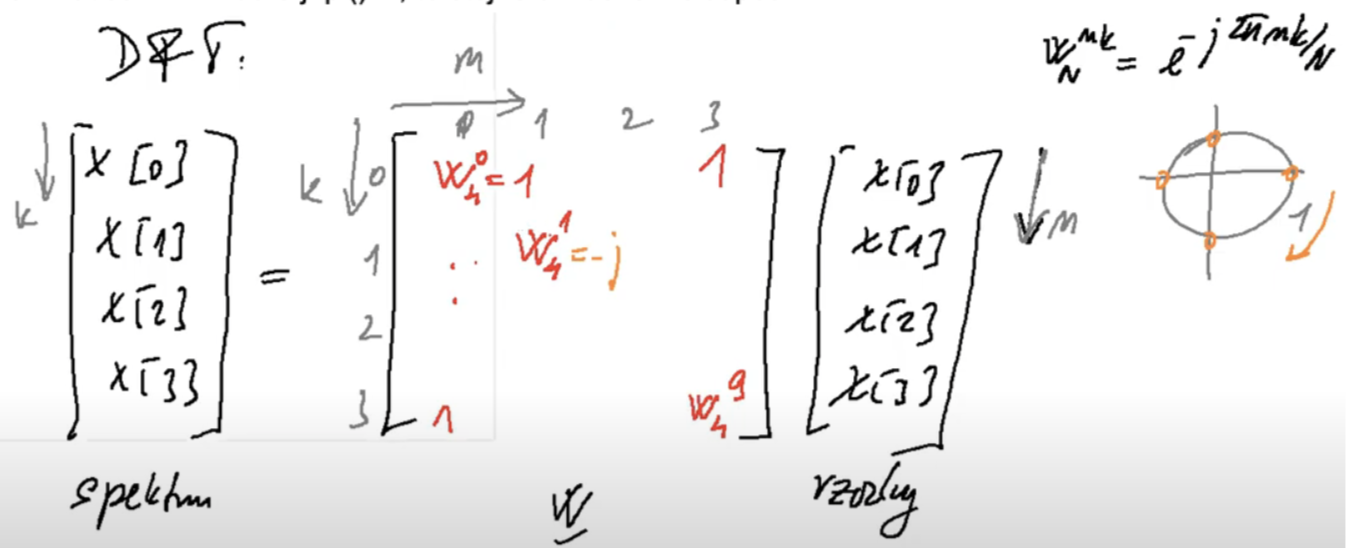
\includegraphics[width=.6\textwidth]{fig/DFT_matrix.png}
\end{figure}
kde \mt{W_N^{nk} = \e^{2\pi n k/N}}. To jsou body na jednotkové kružnici posunuté právě o \mt{\pi/4}, takže jsou na sebe kolmé. 

\begin{center}
        \Ladiesroom~~\Ladiesroom~~\Ladiesroom~~\Ladiesroom~~\Ladiesroom~~\Ladiesroom~~\Ladiesroom~~\Ladiesroom~~\Ladiesroom~~\Ladiesroom~~\Ladiesroom~~\Ladiesroom~~\Ladiesroom~~\Ladiesroom~~\Ladiesroom~~\Ladiesroom~~\Ladiesroom~~\Ladiesroom~~\Ladiesroom~~\Ladiesroom~~\Ladiesroom~~\Ladiesroom~~\Ladiesroom~~\Ladiesroom~~\Ladiesroom~~\Ladiesroom~~\Ladiesroom~~\Ladiesroom~~\Ladiesroom~~\Ladiesroom~~\Ladiesroom~~\Ladiesroom~~\Ladiesroom~~\Ladiesroom~~\Ladiesroom~~\Ladiesroom~~\Ladiesroom~~\Ladiesroom~~\Ladiesroom~~\Ladiesroom~~\Ladiesroom~~\Ladiesroom~~\Ladiesroom~~\Ladiesroom~~\Ladiesroom
\end{center}
        \FloatBarrier

%44
\subsection{Pro jaký typ funkce (signálu) lze ze spojité Fourierovy transformace získat spojitou Fourierovu kosinovou transformaci?}
Pro reálný signál, který ozrcadlíme - prodloužíme tak aby byl sudý. Poté dá sudé reálné spektrum.


%45
\subsection{Vysvětlete principiálně postup úpravy posloupnosti x[n] vedoucí k definici DCT-1 a DCT-2. Jsou tyto transformace ortogonálními trasformacemi?}
Ano, jsou ortogonální. 

DFT sudého a prodlouženého signálu \rrarr DCT
\begin{outline}[enumerate]
        \1 doplnění 2n
        \1 doplnění 2n-1
\end{outline}


%46
\subsection{Jaký je vztah mezi DFT a DCT-1 a jaký mezi DFT a DCT-2. Lze DCT získat pomocí DFT? Jaké úpravy je třeba provést? Stačí vysvětlit slovně nebo s použitím vhodného náčrtku.}

DCT1 - Původní posloupnost doplním nulami, provedu FT, vezmu reálnou část prvních N vzorků, nebo vyrobím sudou posloupnost, udělám DFT o správném rozměru a získám tím DCT.

DFT posloupnost \mt{X_\alpha[k]}, \mt{2N-2} bodů
\begin{align*}
        X_1[k] = 2Re\{X_\alpha[k]\} = 2\sum_{n=0}^{N-1}\alpha[n]x[n]\text{cos}\left(\frac{2\pi kn}{2N+2}\right) = X^{C1}[k]
\end{align*}

idk nějak to tam freestylenu


%47
\subsection{Znáte, kromě DFT a DCT, další ortogonální transformace?}
KLT (PCA), DWT, FT, FS, diskrétní sinová transformace.


\newpage \section{Metoda rozkladu na hlavní komponenty/složky – PCA, EVD, KLT}

\subsection{Popište princip rozkladu signálu na hlavní komponenty (PCA). Co tyto komponenty představují?}
Hledání vlastních čísel a vlastích vektorů. Následně promítneme data ve směru hlavních vektorů. Následně zjišťujeme rozptyl těchto komponent. Pro kompresi bereme tolik, abychom dostali např. 95~\% původní hodnoty.

Hledaný směr rozptylu je shodný se směry hlavních vektorů. Použití pro redukci dimenze. Zjištujeme redundantnost dat

Data centrujeme \rrarr kovarianční matice \rrarr rozklad na \mt{\pmb{VDV}^T}. \mt{\pmb D} je \textit{doagonální} matice s vlastními čísly na diagonále. V je matice, jejíž sloupce tvoří vlastní vektory. 

Používá kovarianční matici \mt{\pmb C_x = \pmb{XX}^T}, kterou následně rozložíme na \mt{\pmb C_x = \pmb{VDV}^T}

Origoš matice \mt{\pmb X} je více měření pod sebou. 



\subsection{Jakou matici PCA používá? Vysvětlete fyzikální význam prvků této matice}
Korelační matice dat, naskládáme naměřená data za sebe -> odhadneme matici korelací. Na diag. rozptyl. Mimo diagonálu - vzájemná energie mezi dvojcí signálů. Pokud nekorelovaná - pouze prvky na hl. diag. 

Úloha hledání vl. čísel a vl. vektorů a průmět dat do směru hlavních vektorů.

Hledání směru s největším ropzylem dat. Hlavní poloosa elipsy. Hlavní komponenta je průmět obláčku do směru daného prvním vlastním vektorem. 

//KLT: původní data krát matice vl. vektorů = dekorelace dat. Nová data kovarianční matice diagonální


%50
\subsection{Na co je rozložena korelační matice pomocí metody PCA?}
Umíme rozložit na součin 3 matic. Prostřední diagonální nenul. prvky na diag, L a P matice vlastních vektorů <- směry největšího rozptylu dat. 

Hledáme takovou tranformaci z ortog. soustavy souřadnic, ve které se nám data promítnou tak, že budou mít co nejvíc energie v nejmenším počtu průmětů. 

Natočíme soustavu tak, aby byl nejdelší rozměr kolineární s jednou ze souřadných os. Zmenšíme dimenzinoalitu. Matice 6ř999s (ze 3 kamer) --> smrsk na 1D úlohu

Diag - vlastní čísla - rozptyl ve směru vl. vektorů


%51
\subsection{Co fyzikálně představují vlastní vektory a vlastní čísla?}
Vl. čísla rozptyl dat ve směru vl. vektorl

Vl. vektory. když do nich natočíme do směrů daných vl. vektory, získáme možnost snížir dimenzinoalitu dat. 1D dat -> info o tom, kolik vl. vektor potřebujeme pro ztrátovou kompresi. 



%52
\subsection{Uveďte příklad, kdy metoda PCA selže. Existuje možnost nápravy?}

Rozložení na kružnici, nemáme význačný směr. Pokud budou data z 1. souboru budou proložena daty z 2. souboru. Lze ošetřit nějakou nelineární transformaci. Kvadrát a tak.

\subsection{Jak lze PCA použít pro ztrátovou kompresi 1-D signálů pomocí KLT (Karhunenovy-Loevovy transformace)?}

1D dat -> info o tom, kolik vl. vektor potřebujeme pro ztrátovou kompresi. 

Stac data, nasegmentujeme, spočteme kovarianční matici  rozložíme na mat. vl. čísel a matice vl. vektor. Data vynásobíme maticí vl. vektorů -> dostaneme nekorelovaný signál. Hodnoty budou seřazeny podle velikosti vlastních čísel. Vezemem tolik hodnot, kolik je vlastních čísel a jejich součet je např. 95 \%. Rekonstrukce signálu - vezmeme transponovanou matici a data dostaneme zpět.


\subsection{Lze pro ztrátovou kompresi použít DCT nebo DFT? V čem se liší postup komprese pomocí DCT nebo DFT od PCA/KLT? Jak se liší dosažitelný stupeň komprese těchto tří metod?}
Ano. PCA, nejlepší komprese. Báze DCT pevná, DFT také. Báze (resp. vlastní vektory) jsou signálově závislé. Dosáhneme optimální kompresi signálu. Nevýhoda - pro každý nový segment signálu nová matice. Výpočetní náročnost. 

\begin{align*}
        \vec{y} = \pmb V \vec{x}
\end{align*}

V praxi DCT

PCA top, DCT mid, DFT low

\subsection{V čem se liší báze DCT či DFT od báze PCA/KLT? Která z těchto metod poskytuje největší kompresní poměr a proč?}
viz předchozí

\subsection{Pomocí čeho se stanovuje počet složek, které použijeme pro ztrátovou kompresi a jak tyto složky vybereme? Porovnejte mezi sebou DFT, DCT a PCA/KLT.}
DFT: vektor signálu, vynásobíme matici sin a cos (W), dostaneme vektor - spektrum, má komplexní čísla, vybereme si taková, která mají největší hodnotu a to přeneseme, ostatní čáry vynulujeme, z přenesených čar provedeme syntézu. Vezmeme iDFT dostaneme rekonstruovaný signál

DCT: jako u DFT

PCA: signálově závislá báze. Hodnoty seřazeny podle velikosti. Matice neobsahuje sin a nebo cos, ale vlastní vektory spočítané z kovarianční matice dat. "spektrum"


\subsection{Co při rozkladu signálu pomocí DFT představují hodnoty modulového spektra |X[k]| nebo výkonového spektra |X[k]|2? Jak se provede ztrátová komprese a následná zpětná rekonstrukce komprimovaného signálu?}

Koeficient podobnosti mezi signálem a jednotlivými komponenty báze. (pomíjíme prosakování). Kvadrát modulu - rozptyl signálu v daném frčním pásmu

Vybereme největší hodnoty spektra, poznamenáme si hodnotu a index, ostatní vynulujeme a přeneseme. Následně sestavíme spektrum a následně použijeme iDFT.

\subsection{Co při rozkladu signálu pomocí DCT představují hodnoty DCT-spektra? Jak se provede ztrátová komprese a následná zpětná rekonstrukce komprimovaného signálu?}

Korelace mezi signálem a cosiny. Ztrátová komprese se dělá obdobně. Porovnání mezi oriho a komprimovaným pomocí střední kvadratické oschylky

\subsection{Co při rozkladu signálu pomocí PCA představují vlastní čísla? Jak se provede ztrátová komprese a následná zpětná rekonstrukce komprimovaného signálu?}

Rozptyly signálu (datové matice) ve směrech danými vlastními vektory.

Komprese identicky, matice je signálově závislá.

vždy:
vezmeme vektor signálu $x$, vynásobíme transformační maticí $T$ (pro DFT a DCT je to $W$, pro PCA je to $W^T$ <- nazýváme KLT), dostaneme $y$, kde jsou nekorelované složky (platí jak pro spektrum, tak pro výsledek KLT (PCA)). Vybereme pouze ty nejsilnější. U KLT je to tolik prvních složek, kde nám dají vlastní čísla v součtu např. 95 \% signálu. U KLT seřazeny podle významnosti.

Následně z $y$ odebereme nevýznamené složky a dostaneme $\tilde{y}$. následně $\tilde{y}\,\cdot\,T^{-1}~=~\tilde{x}$, kde $T^-1~=~W^{-1}$, nebo $V$. 

Chyba aproximace $e[n]~=~x[n] - \tilde{x}[n]$.

Matici $V^T$ získáme metodou PCA a nebo EVD (eigen value decomposition) $\leftrightarrow$ $C_x \rightarrow V, D$


%%%%%%%%%%%%%%%%%%%%%%%%%%%%%%%%%%%%%%%%%%%%%%%%%%%%%%%%%%%%%%%%%%%%%%%%%%%%%%%%%%%%%%%%%%%%
%60 - 67
\newpage \section{Modely zkreslení signálu a možnosti jeho rekonstrukce – inverzní filtrace}
%60
\subsection{Načrtněte model a napište rovnice pro zkreslení signálu aditivním šumem – rovnice napište pro časovou oblast, pomocí korelací i spektrálních hustot.}

Časová oblast:
\begin{align*}
        y[n] = s[n] + u[n]
\end{align*}

Korelační oblast:
\begin{align*}
        R_x[k] = R_s[k] + R_u[k]
\end{align*}

PSD:
\begin{align*}
        S_x(\ejt) = S_s(\ejt) + S_u(\ejt)
\end{align*}


%61
\subsection{Načrtněte model a napište rovnice pro zkreslení signálu konvolučním šumem – rovnice napište pro časovou oblast, pomocí korelací i spektrálních hustot.}
\begin{align*}
        y[n] = s[n]\ast u[n]
\end{align*}

Pro korelaci signálu zkresleného konvolucí platí:
\begin{align*}
        R_x[k] = R_s[k]\ast R_h[k]
\end{align*}

Pro PSD signálu zkresleného konvolucí platí
\begin{align*}
        S_x(ejt) = S_s(ejt)|H(\ejt)|^2
\end{align*}


%62
\subsection{Načrtněte model a napište rovnice pro zkreslení signálu aditivním a konvolučním šumem – rovnice napište pro časovou oblast, pomocí korelací i spektrálních hustot.}

Spojení těch rovnic nahoře


%63
\subsection{Jak lze potlačit aditivní šum?}
Pokud široko/úzkopásomový, tak ezy filtr. 

Nebo odhadneme spektrum šumu a ve spektrální oblasti ho odečteme.


%64
\subsection{Jak lze potlačit konvoluční šum?}

Lineární:
\begin{outline}
        \1 prostá dekonvoluce
        \1 pseudoinverze (nulování slabých spektrálních čar)
        \1 Wienerova filtrace 
        \1 adaptivní metody
\end{outline}

Nelineární:
\begin{outline}
        \1 nelinearita bez paměti - redukce odlehlých hodnot
        \1 nelinearita s pamětí - kombinace LTI filtru s pamětí a mediánového filtru
\end{outline}


%65
\subsection{Vysvětlete princip a vlastnosti prosté inverzní filtrace.}

hardcore matika ahead!!
\begin{align*}
        H_i = \frac{1}{H}
\end{align*}

Kde \mt{H_i} je inverzní přenos přenosu systému, přes který signál prošel.

Prostě signál projde přes nějaký systém s přenosem, tak hledáme inverzní přenos, abychom zpátky dohnali ztracené spektrální vlastnosti. 

Problémosy:
\begin{outline}
        \1 vliv šumu \rrarr šumová katastrofa
        \1 neminimální fáze \rrarr problém stability
\end{outline}



\subsection{Co znamená pojem šumová katastrofa a kdy k ní dochází? Vysvětlete pro deterministické signály. Jak ji lze potlačit?}

Vzinká při metodě zvýrazňování signálu - u prosté dekonvoluce inverzním filtrem
když má filtr nuly vně jednotkové kružnice, tak jakmile udělám inverzní, začne vlastně místo zeslabování šumu ho zesilovat, to je šumová katastrofa.

Řešení: oprahujeme přenosovou charakteristiku.


%67
\subsection{Jaké existují modifikace inverzní filtrace? Napište příslušné vztahy pro inverzní filtraci, které objasní šumovou katastrofu a popíší modifikace inverzní filtrace (lze použít deterministický popis).}
\textbf{Pseudoinverze}:
\begin{align*}
        H_I = 1/H \text{ pro } [1/H] < M, H_I = 0 \text{ pro } [1/H] \geq M 
\end{align*}

\textbf{Limitace}:
\begin{align*}
        H_I = 1/H \text{ pro } [1/H] < M, H_I = H\e^{j\text{arg}(1/H)} \text{ pro } [1/H] \geq M
\end{align*}




%68 - 71
\newpage \section{Slepá separace a dekonvoluce}

%68
\subsection{Jaké dva základní způsoby učení/trénování adaptivních filtrů nebo klasifikačních algoritmů znáte? Vysvětlete princip a rozdíly.}

\begin{outline}
        \1 Učení s učitelem - existují trénovací signálu, pro které známe požadovanou odezvu systému
        \1 Učení bez učitele - slepá adaptace - neexistuje trénovací signál, ale existuje požadovaný soubor pravidel umožňující nastavit specifický vztah mezi vstupem a výstupem. 
\end{outline}


%69
\subsection{Jaké jsou předpoklady pro slepou separaci signálů/zdrojů? Jaké jsou předpoklady pro slepou dekonvoluci ?}

Předpoklady:
\begin{outline}
        \1 lineární kombinace \mt{x_i(t)} signálů \mt{s_i(t)}
        \1 nezávislé signály \mt{s_i(t)}
\end{outline}
\begin{align*}
        \vec{x}(t) = \pmb A \vec s(t)
\end{align*}

Pro rozdělení:
\begin{align*}
        \vec{y}(t) = \pmb W \vec x(t) =  \pmb W\pmb A \vec s(t) = \pmb D \pmb P \vec s(t),
\end{align*}

kde \mt{\pmb W} je matice separace, složená z diagonální \mt{\pmb D} a permutační \mt{\pmb P} matice (prohazuje řádky). 

%70
\subsection{Čím se liší slepá separace od slepé dekonvoluce? K čemu slouží obě metody? Do které skupiny patří metoda nazývaná FastIca?}

Slepá dekonvoluce - známe pouze \textbf{výstupní signál}, může být přítomen aditivní šum. Snažíme se minimalizovat vliv \mt{h(t)} systému. 

Slepá separace - máme směs signálů, snažíme se najít jednotlivé prvky signálu.

FastICA - separace.


%71
\subsection{Jaké dekonvoluční metody jsme v tomto kursu poznali? čím se od sebe liší a jaké jsou jejich předpoklady pro úspěšnou dekonvoluci?}

\begin{outline}
        \1 PCA - \textit{Principal Component Analysis} - hledá směry největšího rozptylu dat (statistika druhého řádu)
        \1 ICA - \textit{Independent Component Analysis} - využívá statistiky vyšších řádů.
\end{outline}



%72 - 84 
\newpage \section{Vlnková transformace – spojitá CWT, diskrétní DWT, banka filtrů, kvadraturní zrcadlové filtry}

\subsection{Vysvětlete postup analýzy signálu pomocí FT a STFT. Jak se jmenují výstupy obou metod a co fyzikálně představují?}
Dyž FT, tak Spektrum\\
Dyž STFT, tak Spektrogram\\
Pyčo!

Princip STFT:\\
signál je nasegmentován na krátké časové úseky a pro každý segment (a jeho překryvy) se udělá vyhlazený spektrální odhad PWelch. Tímto je získán 2D graf, který znázorňuje vývoj PDS v čase (spektrogram).


\subsection{Jaký je základní rozdíl mezi STFT a CWT?}
\sout{STFU} STFT: signál porovnáváme s harmonickým průběhem

CWT: na výběr máme sadu předem daných vlnek, které porovnáváme se signálem. 

%74
\subsection{Jak vypadá časově-frekvenční rozlišení pro STFT a DWT?}
STFT - Konstantní poměr frekvenčního a časového rozlišení: \mt{\Delta f = 1/T_0}.

\begin{figure}[h]
        \centering
        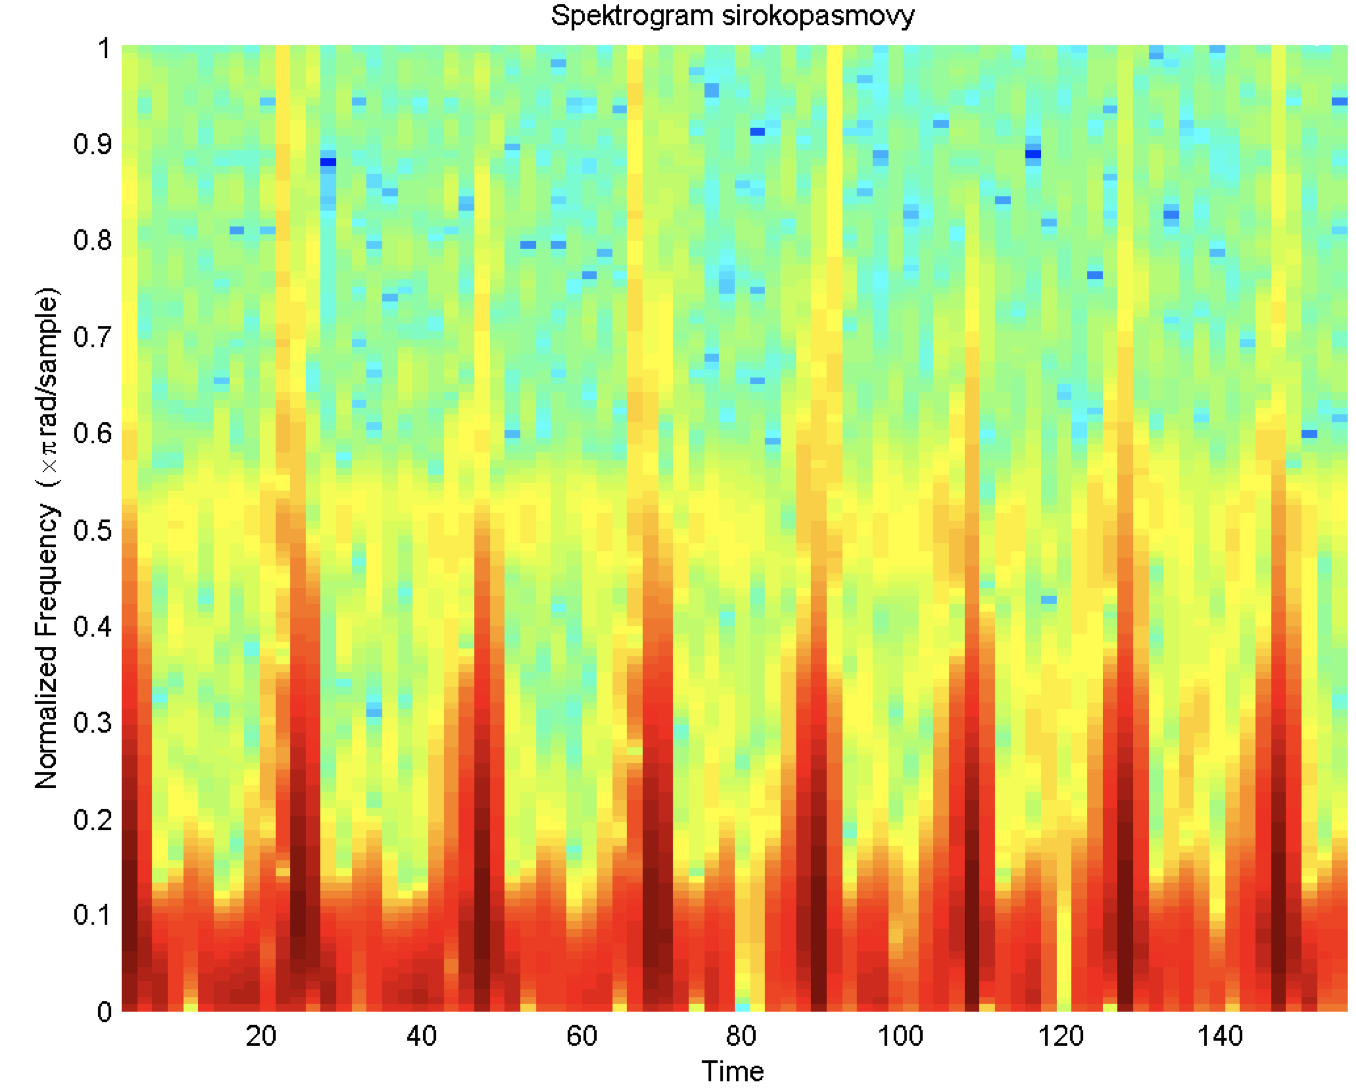
\includegraphics[width=.5\textwidth]{fig/spectrogram.png}
        \caption*{Spectrogram: měníme frekvenci porovnávané funkce (STFT)}
\end{figure}
\begin{figure}[h]
        \centering
        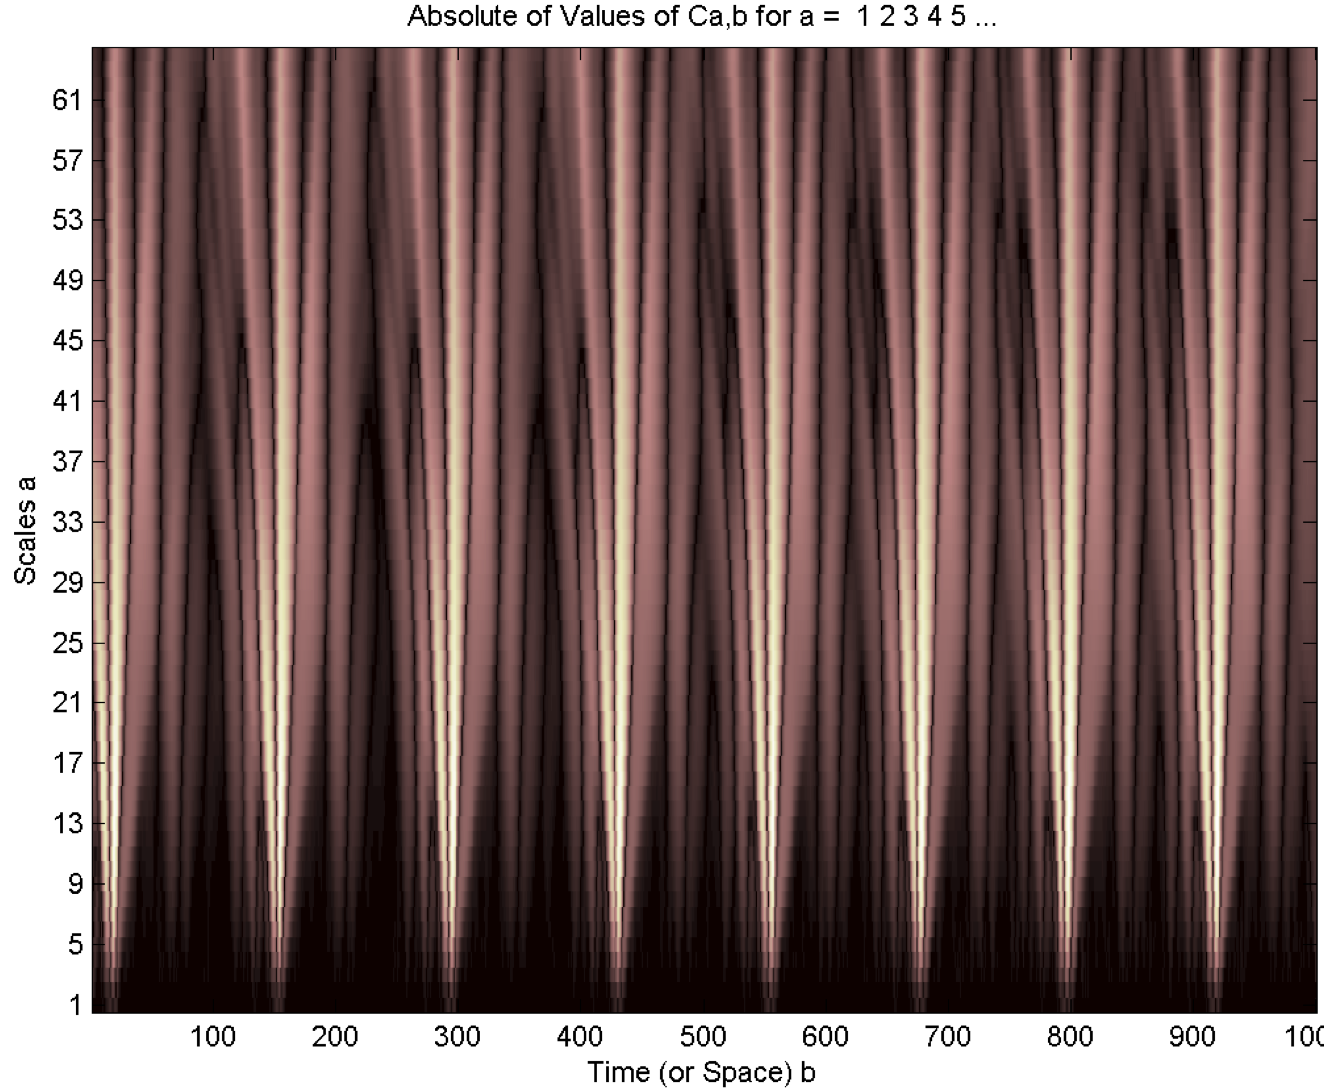
\includegraphics[width=.5\textwidth]{fig/scalogram.png}
        \caption*{Scalogram: měníme časové škálování (roztažení) vlnky (CWT)}
\end{figure}
\FloatBarrier

%75
\subsection{Co znamenají pojmy vlnka, hladina, aproximace a detaily? Uveďte vhodný příklad s náčrtkem pro vysvětlení těchto pojmů.}
Vlnka: bázová funkce tranformace. Můžeme roztahovat v čase

Hladina: hodnota koeficientu roztažení

Pokud signál proženeme horní a dolní propustí, dostaneme aproximace a detaily

$x[n]~\rightarrow~\text{DP, decimace 2}~\rightarrow~\text{aproximace - }c_j$\\
$x[n]~\rightarrow~\text{HP, decimace 2}~\rightarrow~\text{detaily - }d$

Detailní signál lze získat řezem na dané hladině


%76
\subsection{čím se liší CWT od DWT? K čemu se používají?}
DWT se smrskává pomocí decimace signálu. Posun i měřítko jsou mocniny dvou.

Má rodinu vlnek, která se odvozuje z mateřské vlnky.

Používá sumu místo integrálu

\begin{figure}
        \centering
        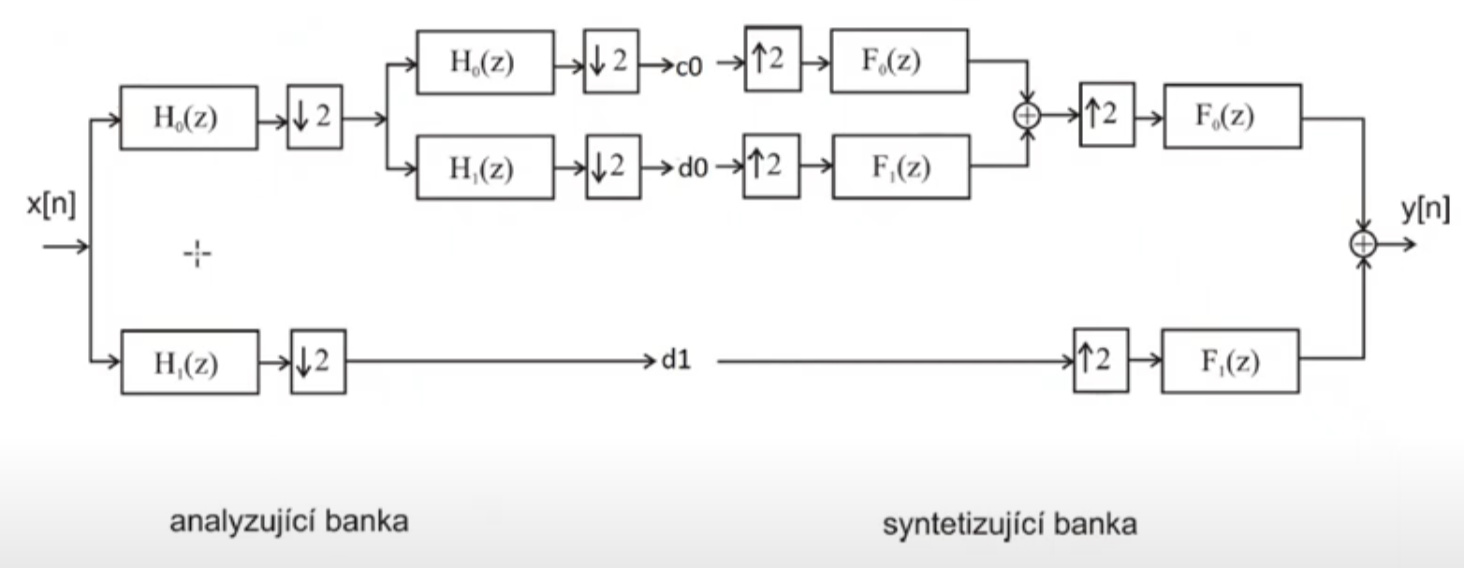
\includegraphics[width=.8\textwidth]{fig/DWT_blokac.png}
        \caption*{Prolly blokáč DWT}
\end{figure}

Poté vidíme signály na jednotlivých hladinách, lze jednoduše odstranit šum, komprimovat podle důležitých hladin. Přibližování v efektivitě metodě KLT, ale nemusíme opakovaně počítat bázi. Stonks dpč. 


%77
\subsection{Co znamenají pojmy měřítková funkce a měřítková rovnice, vlnka a vlnková rovnice? Uveďte libovolný příklad pro vysvětlení těchto pojmů a vztahů mezi nimi.}
Měřítková funkce - funkce, ze které je možné odvodit mateřskou vlnku banky filtrů. 

implementace DWT pomocí banky filtrů.

vlnka je nějaký přechodový děj (tranzienta), nulová střední hodnota, konečná energie.

Měřítková rovnice:
\begin{align*}
        \phi(t) = \sqrt{2} \sum h_0[n]\phi(2t-n),
\end{align*}
kde \mt{\phi (t)} je měřítková funkce a \mt{h_0} jsou koeficienty rekonstrukční dolní propusti. Vlnková rovnice generuje vlnky pomocí konvoluce měřítkové funkce s koeficienty rekonstrukční horní propusti. 


%78
\subsection{Načrtněte banku filtrů, která realizuje DWT. Jak impulsové odezvy použitých filtrů souvisejí s měřítkovou funkcí a vlnkou?}
\begin{figure}
        \centering
        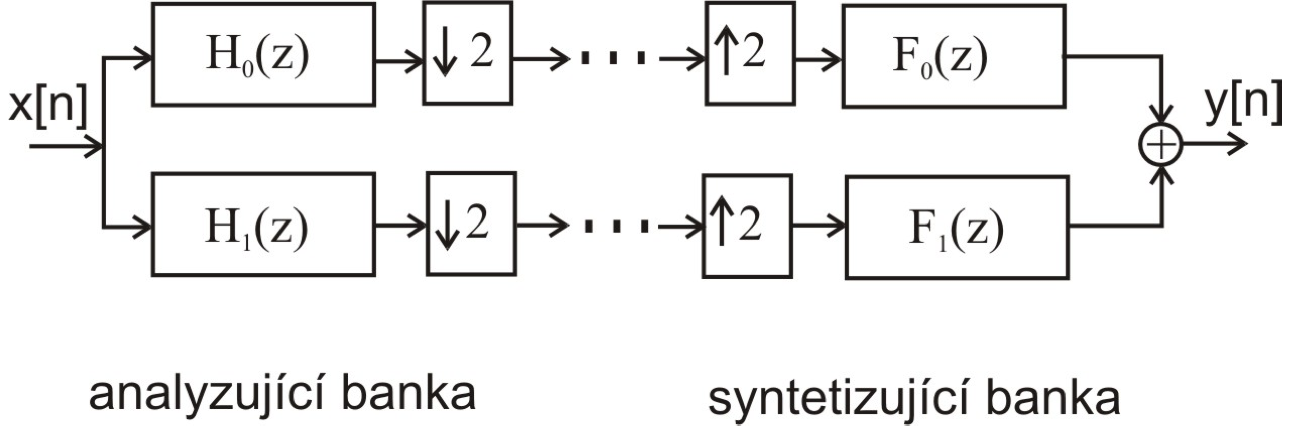
\includegraphics[width=.6\textwidth]{fig/banka_filtru.png}
        \caption*{Dvoupásmová banka filtrů}
\end{figure}

\begin{outline}
        \1 \textbf{Aproximace}: výstup DP 
        \1 \textbf{Detaily}: výstup HP
        \1 \textbf{Analyzující banka filtrů}: rozklad signálu do pásem a decimace
        \1 \textbf{Syntetizující banka filtrů}: interpolace a sloučení signálu.
\end{outline}

Nutno aby nedošlo ke zkreslení signálu a překrývání. 


%79
\subsection{Vysvětlete princip základního způsobu redukce šumů pomocí DWT. Co znamená měkké a tvrdé prahování?}

Rozložíme na koeficienty pomocí banky filtrů a šum redukujeme nulováním hodnot pod daným prahem (nebo brnem (haha(ah(aaa(je půlnoc (v NTKčku) před zkouškou (dneska mám zkoušku (boha, kdy se to mám naučit (asi příští semestr)))))))). 

Tvrdé prahování - oříznutí hodnoty pod daným prahem\\
Měkké prahování (brnování, páč tam jsou měkký) - pokud překročíme práh, tak hodnotu pouze snížíme, nevynulujeme



%80
\subsection{Co znamená termín mateřská vlnka? Znáte nějaké typy těchto vlnek?}

Základní vlna, ze které jsou posléze vytvářeny dceřiné vlnky. 

Mexická vlnka, Haarova, Morletova.


%81
\subsection{Jak probíhá redukce šumu pomocí STFT a jak pomocí DWT?}

Ořezáváme spectrogramy/scalogramy tam, kde by mohl být šum a provedem zpětnou tranformaci. U CWT bude šum prolly v detailech. 


%82
\subsection{Načrtněte dvoupásmovou banku filtrů a vysvětlete následující pojmy: analyzující a syntetizující banka filtrů, perfektní rekonstrukce a důsledek požadavku perfektní rekonstrukce pro filtry použité v bance filtrů. Proč se v bance filtrů používá decimace a interpolace?}
Dvoupásmová - dělení pásma na dvě poloviny DP/HP, zrcadlové filtry. 

Kvadraturní zrcadlové filtry - výkonově komplementární \
\begin{align*}
        |H_0(\ejt)|^2 + |H_1(\e^{j(\theta-\pi)})|^2 = 1
\end{align*}

Decimací a doplněním nulami se obohatí spektrum \rrarr vznik zrcadel.


$x[n]~\rightarrow~\text{DP, decimace 2}~\rightarrow~\text{aproximace - }c_j$\\
$x[n]~\rightarrow~\text{HP, decimace 2}~\rightarrow~\text{detaily - }d$

\begin{figure}[h!]
        \centering
        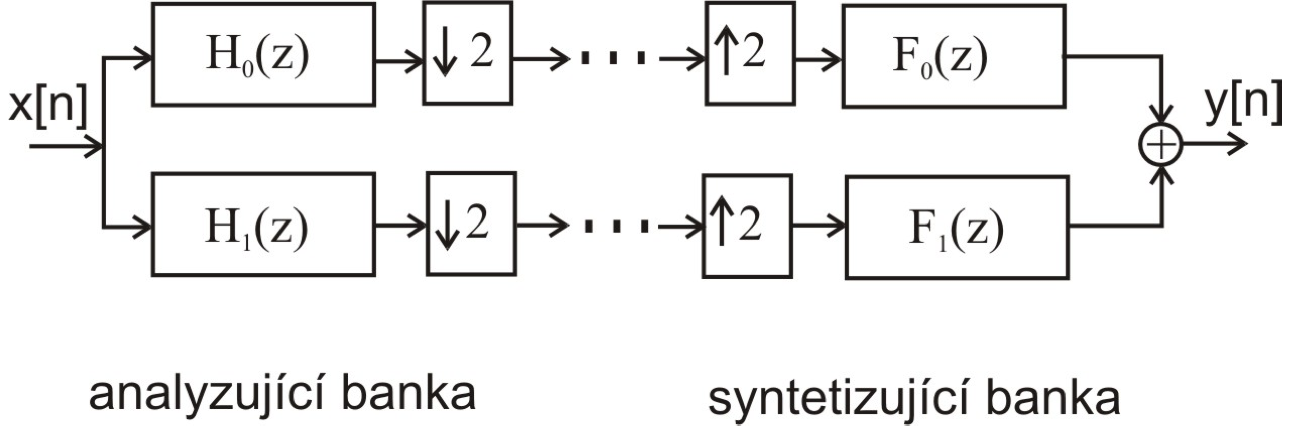
\includegraphics[width=.7\textwidth]{fig/banka_filtru.png}
        \caption*{Dvoupásmová mamka filtrů}
\end{figure}

Perfektní rekonstrukce - filtry jsou oproti sobě zrcadlově a výkonově symetrická.

Podmínky:
\begin{outline}
        \1 Žádné překrývání
        \1 Žádné zkreslení
\end{outline}

\FloatBarrier
%83
\subsection{Vysvětlete stručně postup návrhu dvoupásmové banky filtrů s perfektní rekonstrukcí. Jsou přenosové funkce filtrů použitých v dvoupásmové bance filtrů libovolné nebo jsou vázány nějakými podmínkami?}

\begin{outline}[enumerate]
        \1 Návrh prototypu \mt{H_0(z)}
        \1 Pomocí rovnic odvodíme zbytek filtrů
                \2 Filtry se budou hezky překrývat (kauzalita zakazuje ostré hrany)
        \1 Návrh filtru od 0 do fs/4 a od fs/4 do fs/2
                \2 nutná výkonová komplementárnost
\end{outline}



%84
\subsection{Vysvětlete pojem kvadraturní zrcadlové filtry a načrtněte jejich frekvenční charakteristiky.}

Filtry, které jsou proto sobě zrcadlové a mají stejné výkonové zesílení. Součet kvadrátu modulu musí dát 1. 

Výkonově komplementární \mt{\leftrightarrow} kvadraturní zrcadlové filtry

Pokud nepotřebujeme perfektní rekonstrukci, lze použít i FIR filtry.

\begin{figure}[h!]
        \centering
        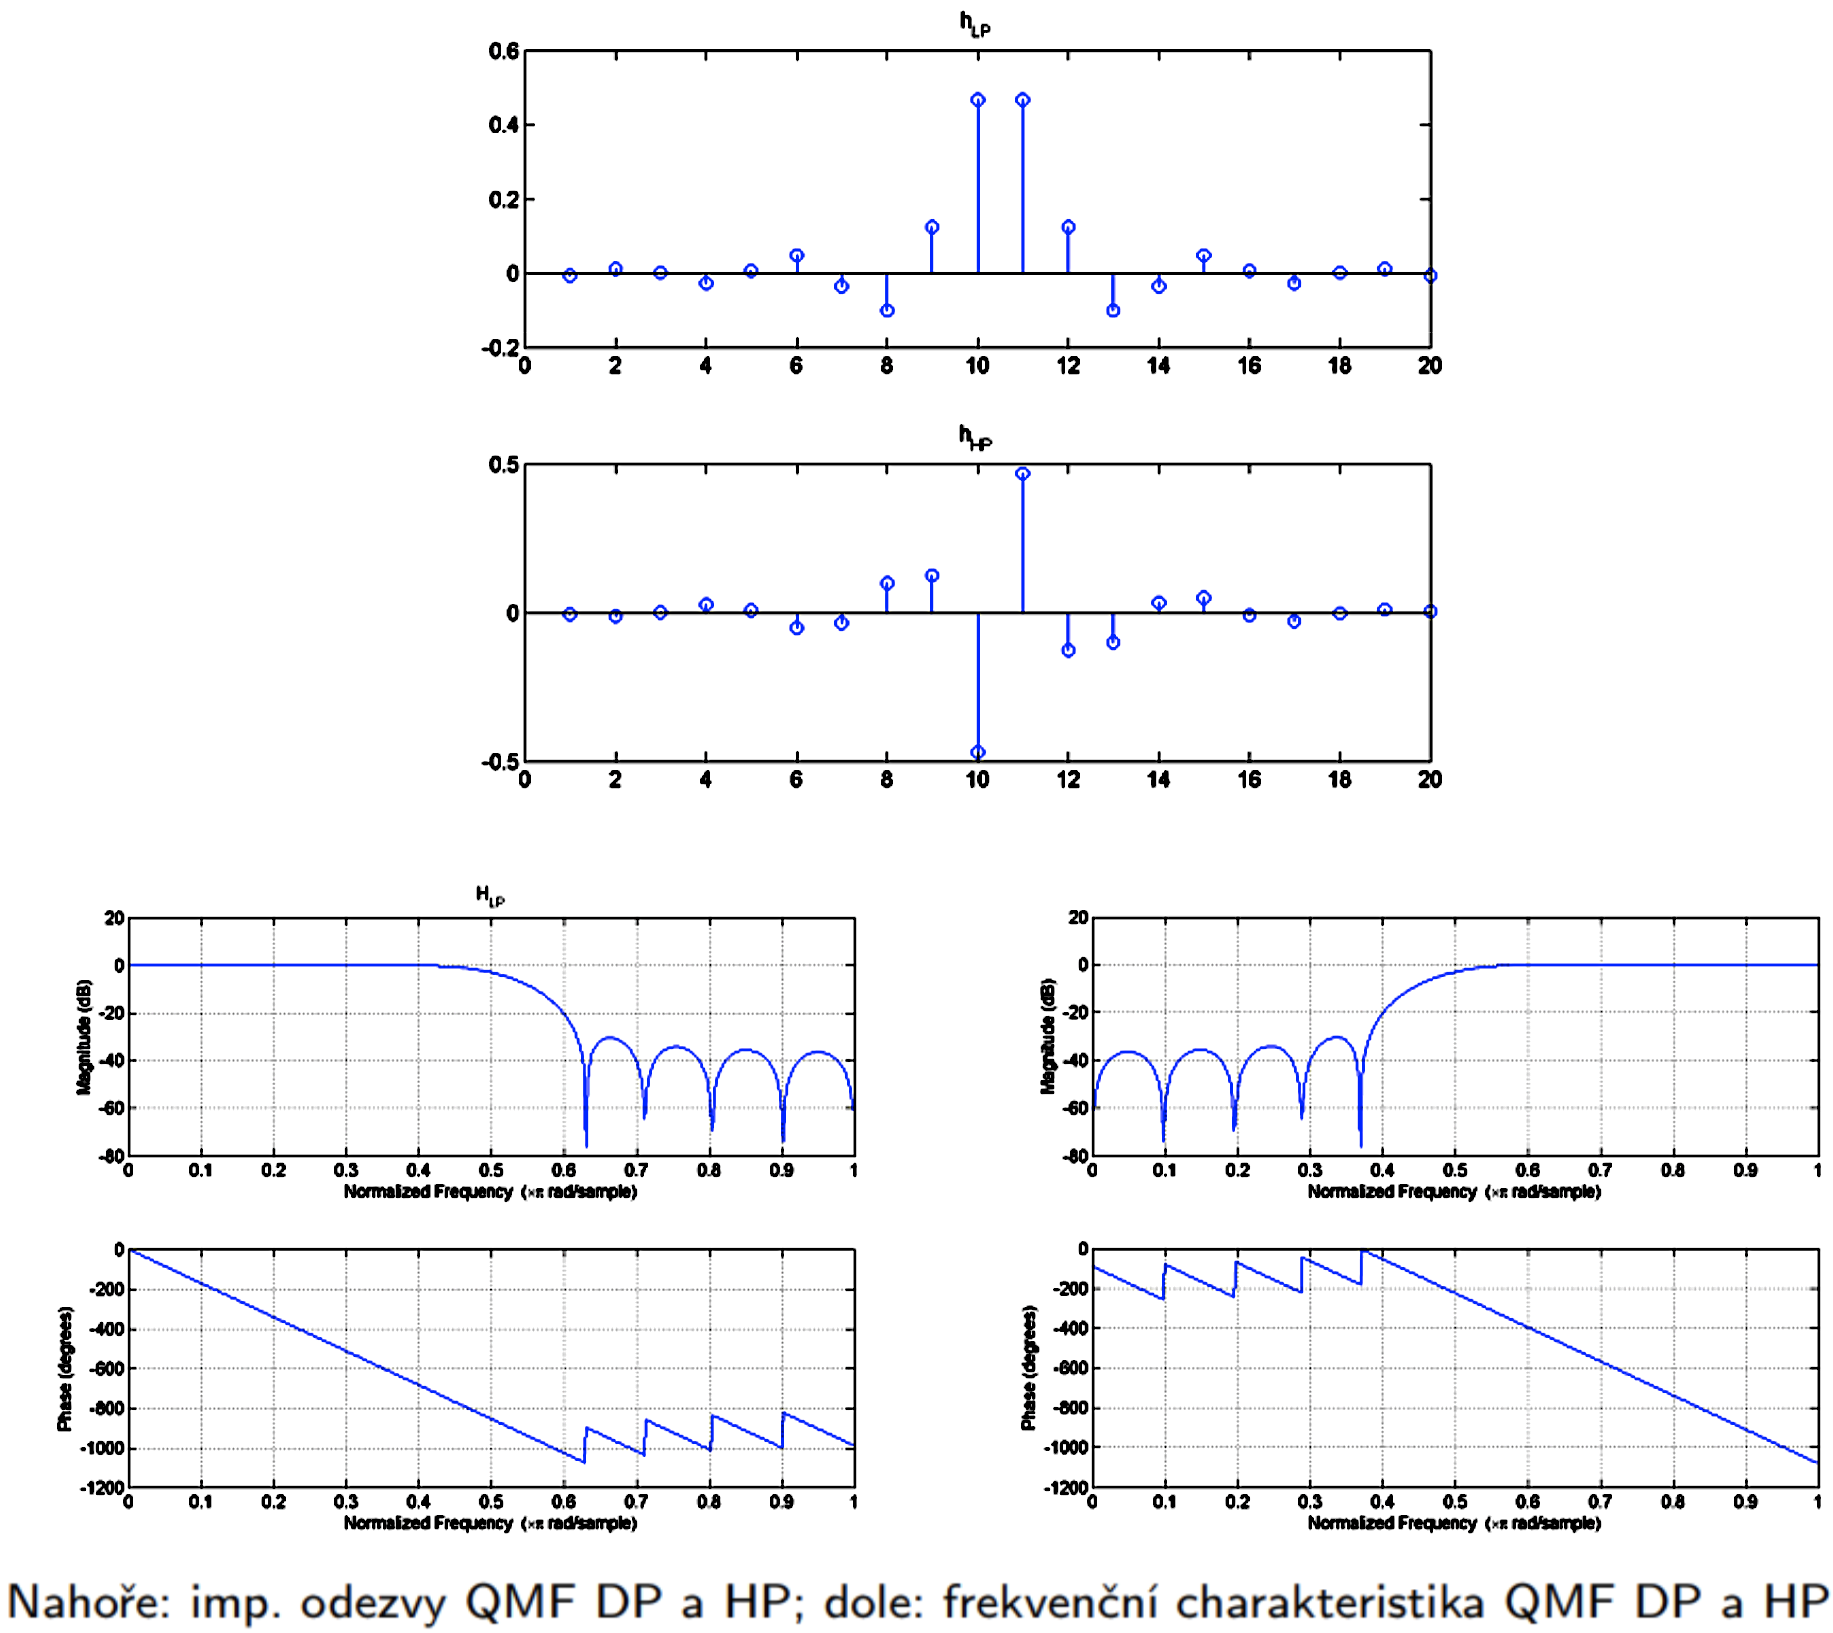
\includegraphics[width=.9\textwidth]{fig/qmf.png}
\end{figure}
\FloatBarrier
\vfill
\begin{flushright}
        Konec zvonec\\
        Běžte domu, tady už se nic nedozvíte
\end{flushright}
\end{document}




